% Options for packages loaded elsewhere
\PassOptionsToPackage{unicode}{hyperref}
\PassOptionsToPackage{hyphens}{url}
%
\documentclass[
]{article}
\usepackage{amsmath,amssymb}
\usepackage{iftex}
\ifPDFTeX
  \usepackage[T1]{fontenc}
  \usepackage[utf8]{inputenc}
  \usepackage{textcomp} % provide euro and other symbols
\else % if luatex or xetex
  \usepackage{unicode-math} % this also loads fontspec
  \defaultfontfeatures{Scale=MatchLowercase}
  \defaultfontfeatures[\rmfamily]{Ligatures=TeX,Scale=1}
\fi
\usepackage{lmodern}
\ifPDFTeX\else
  % xetex/luatex font selection
\fi
% Use upquote if available, for straight quotes in verbatim environments
\IfFileExists{upquote.sty}{\usepackage{upquote}}{}
\IfFileExists{microtype.sty}{% use microtype if available
  \usepackage[]{microtype}
  \UseMicrotypeSet[protrusion]{basicmath} % disable protrusion for tt fonts
}{}
\makeatletter
\@ifundefined{KOMAClassName}{% if non-KOMA class
  \IfFileExists{parskip.sty}{%
    \usepackage{parskip}
  }{% else
    \setlength{\parindent}{0pt}
    \setlength{\parskip}{6pt plus 2pt minus 1pt}}
}{% if KOMA class
  \KOMAoptions{parskip=half}}
\makeatother
\usepackage{xcolor}
\usepackage[margin=1in]{geometry}
\usepackage{graphicx}
\makeatletter
\def\maxwidth{\ifdim\Gin@nat@width>\linewidth\linewidth\else\Gin@nat@width\fi}
\def\maxheight{\ifdim\Gin@nat@height>\textheight\textheight\else\Gin@nat@height\fi}
\makeatother
% Scale images if necessary, so that they will not overflow the page
% margins by default, and it is still possible to overwrite the defaults
% using explicit options in \includegraphics[width, height, ...]{}
\setkeys{Gin}{width=\maxwidth,height=\maxheight,keepaspectratio}
% Set default figure placement to htbp
\makeatletter
\def\fps@figure{htbp}
\makeatother
\setlength{\emergencystretch}{3em} % prevent overfull lines
\providecommand{\tightlist}{%
  \setlength{\itemsep}{0pt}\setlength{\parskip}{0pt}}
\setcounter{secnumdepth}{-\maxdimen} % remove section numbering

\newcommand{\beginsupplement}{%
        \setcounter{table}{0}
        \renewcommand{\thetable}{S\arabic{table}}%
        \setcounter{figure}{0}
        \renewcommand{\thefigure}{S\arabic{figure}}%
     }

\usepackage{lineno}
\linenumbers

\usepackage[compress, super]{natbib}

\usepackage{setspace} \doublespacing

\usepackage{siunitx}

\usepackage[utf8]{inputenc}
\usepackage{amsmath}
\usepackage{algorithm}
\usepackage{algpseudocode}

\algrenewcommand\algorithmicrequire{\textbf{Input:}}
\algrenewcommand\algorithmicensure{\textbf{Output:}}
\ifLuaTeX
  \usepackage{selnolig}  % disable illegal ligatures
\fi
\IfFileExists{bookmark.sty}{\usepackage{bookmark}}{\usepackage{hyperref}}
\IfFileExists{xurl.sty}{\usepackage{xurl}}{} % add URL line breaks if available
\urlstyle{same}
\hypersetup{
  pdftitle={Transcripts with high distal heritability mediate genetic effects on complex traits},
  hidelinks,
  pdfcreator={LaTeX via pandoc}}

\title{Transcripts with high distal heritability mediate genetic effects
on complex traits}
\author{}
\date{\vspace{-2.5em}}

\begin{document}
\maketitle

Anna L. Tyler, J. Matthew Mahoney, Mark P. Keller, Candice N. Baker,
Margaret Gaca, Anuj Srivastava, Isabela Gerdes Gyuricza, Madeleine
Braun, Nadia A. Rosenthal, Alan D. Attie, Gary A. Churchill and Gregory
W. Carter

\subsection{Abstract}\label{abstract}

Although many genes are subject to local regulation, recent evidence
suggests that complex distal regulation may be more important in
mediating phenotypic variability. To assess the role of distal gene
regulation in complex traits, we combined multi-tissue transcriptomes
with physiological outcomes to model diet-induced obesity and metabolic
disease in a population of 371 Diversity Outbred mice. Using a novel
high-dimensional mediation analysis, we identified a composite
transcriptome signature that summarized genetic effects on gene
expression and explained 30\% of the variation across all metabolic
traits. The signature was heritable, interpretable in biological terms,
and predicted obesity status from gene expression in an independently
derived mouse cohort and multiple human studies. Transcripts
contributing most strongly to this composite mediator frequently had
complex, distal regulation distributed throughout the genome. These
results suggest that trait-relevant variation in transcription is
largely distally regulated, but is nonetheless identifiable,
interpretable, and translatable across species.

\subsection{Introduction}\label{introduction}

In the quest to understand the genetic architecture of complex traits,
gene expression is an important mediator between genotype and phenotype.
There is ample evidence from genome-wide association studies (GWAS) that
regulation of gene expression accounts for the bulk of the genetic
effect on complex traits, as most trait-associated variants lie in gene
regulatory regions \cite{pmid22955828, 
pmid25363779, pmid21617055, pmid19474294, pmid24702953, 
pmid24316577, pmid27126046}. It is widely assumed that these variants
influence local transcription, and methods such as transcriptome-wide
association studies (TWAS)
\cite{pmid33020666, pmid26258848, pmid27019110, pmid26854917} and
summary data-based Mendelian randomization (SMR) \cite{pmid27019110}
capitalize on this idea to identify genes associated with multiple
disease traits \cite{pmid29567659, pmid35533209, 
pmid27309819, pmid30950127}

Despite the great promise of these methods, explaining trait effects
with local gene regulation has been more difficult than initially
assumed \cite{pmid32912663, pmid36515579}. Although trait-associated
variants tend to lie in non-coding, regulatory regions, they often do
not have detectable effects on gene expression \cite{pmid32912663} and
tend not to co-localize with expression quantitative trait loci (eQTLs)
\cite{pmid36515579, pmid37857933}.

One possible explanation for these observations is that gene expression
is not being measured in the appropriate cell types and thus local eQTLs
influencing traits cannot be detected \cite{pmid32912663}. An
alternative explanation that has been discussed in recent years is that
effects of these variants are mediated not through local regulation of
gene expression, but through distal regulation
\cite{pmid37857933, pmid32424349, 
pmid32831138, pmid30950127}. In this model, a gene's expression is
influenced by many variants throughout the genome through their
cumulative effects on a broader regulatory network. In other words, the
heritable component of the transcriptome is an emergent state arising
from the myriad molecular interactions defining and constraining gene
expression.

To assess the role of wide-spread distal gene regulation on complex
traits, we investigated diet-induced obesity and metabolic disease as an
archetypal example. Diet-induced obesity and metabolic disease are
genetically complex with hundreds of variants mapped through GWAS
\cite{pmid36350656, 
pmid34556834}. These variants are known to act through multiple tissues
that interact dynamically with each other
\cite{pmid28089486, pmid10889786}, including adipose tissue, pancreatic
islets, liver, and skeletal muscle. The multi-system etiology of
metabolic disease complicates mechanistic dissection of the genetic
architecture, requiring large, dedicated data sets that include
high-dimensional, clinically relevant phenotyping, dense genotyping in a
highly recombined population, and transcriptome-wide measurements of
gene expression in multiple tissues.

Measuring gene expression in multiple tissues is critical to adequately
assess the extent to which local gene regulation varies across the
tissues and whether such variablilty might account for previous failed
attempts to identify trait-relevant local eQTL. Such data sets are
extremely difficult to obtain in human populations, particularly in the
large numbers of subjects required for adequate statistical power. Thus,
to further investigate the role of local and distal gene regulation on
complex traits, we generated two complementary data sets: A discovery
data set in a large population of diversity outbred (DO) mice
\cite{pmid22892839}, and an independent validation data set derived by
crossing inbred strains from the Collaborative Cross (CC) mice
\cite{pmid18716833} to form CC F1 mice (CC-RIX). Both populations
modeled diet-induced obesity and metabolic disease \cite{pmid29567659}.

The DO population and CC recombinant inbred lines were derived from the
same eight inbred founder mouse strains, five classical lab strains, and
three strains more recently derived from wild mice \cite{pmid22892839}.
They represent three subspecies of mouse
\textit{Mus musculus domesticus}, \textit{Mus musculus musculus}, and
\textit{Mus musculus casteneus}, and capture 90\% of the known variation
in laboratory mice \cite{pmid31133439}. The DO mice are maintained with
a breeding scheme that ensures equal contributions from each founder
across the genome thus rendering almost the whole genome visible to
genetic inquiry \cite{pmid22892839}. The CC mice were initially
outcrossed to recombine the genomes from all eight founders, and then
inbred for at least 20 generations to generate multiple inbred lines.
Because these two populations have common ancestral haplotypes, we could
directly and unambiguously compare the local genetic effects on gene
expression at the whole-transcriptome level while varying the population
structure driving distal regulation.

In the DO population, we paired clinically relevant metabolic traits
from 371 mice \cite{pmid29567659}, including body weight, plasma levels
of insulin, glucose and lipids, with transcriptome-wide gene expression
in four tissues related to metabolic disease: adipose tissue, pancreatic
islets, liver, and skeletal muscle. We measured similar metabolic traits
in a CC-RIX population and gene expression from three of the four
tissues used in the DO: adipose tissue, liver, and skeletal muscle.
Because the CC-RIX carry the same founder alleles as the DO, local gene
regulation is expected to match between the populations, but because the
alleles are recombined through the genome, distal effects are expected
to vary from those in the DO, allowing us to directly assess the role of
local gene regulation in driving trait-associated transcript variation.
Together, these data enable a comprehensive view into the genetic
architecture of metabolic disease.

\subsection{Results}\label{results}

To comprehensively assess the genetic control of gene expression in
metabolic disease in mice, we assayed metabolic traits and multi-tissue
gene expression in DO mice.

\subsubsection{Genetic variation contributed to wide phenotypic
variation}\label{genetic-variation-contributed-to-wide-phenotypic-variation}

Although the environment was consistent across the DO mice, the genetic
diversity present in this population resulted in widely varying
distributions across physiological measurements (Fig.
\ref{fig:trait_overview}). For example, body weights of adult
individuals varied from less than the average adult C57BL/6J (B6) body
weight to several times the body weight of a B6 adult in both sexes
(Males: 18.5 - 69.1g, Females: 16.0 - 54.8g) (Fig.
\ref{fig:trait_overview}A). Fasting blood glucose (FBG) also varied
considerably (Fig. \ref{fig:trait_overview}B), although few of the
animals had FBG levels that would indicate pre-diabetes (19 animals,
3.8\%), or diabetes (7 animals, 1.4\%) according to previously developed
cutoffs (pre-diabetes: FBG \(\geq\) 250 mg/dL, diabetes: FBG \(\geq\)
300, mg/dL) \cite{pmid17018838}. Males had higher FBG than females on
average (Fig. \ref{fig:trait_overview}C) as has been observed before
suggesting either that males were more susceptible to metabolic disease
on the high-fat, high-sugar (HFHS) diet, or that males and females may
require different thresholds for pre-diabetes and diabetes.

Body weight was strongly positively correlated with food consumption
(Fig. \ref{fig:trait_overview}D \(R^2 =\) 0.51, \(p<\)
\ensuremath{2.2\times 10^{-16}}) and FBG (Fig.
\ref{fig:trait_overview}E, \(R^2=\) 0.21, \(p <\)
\ensuremath{2.2\times 10^{-16}}) suggesting a link between behavioral
factors and metabolic disease. However, the heritability of this trait
and others (Fig. \ref{fig:trait_overview}F) indicates that genetics
contribute substantially to correlates of metabolic disease in this
population.

\begin{figure}[ht!]
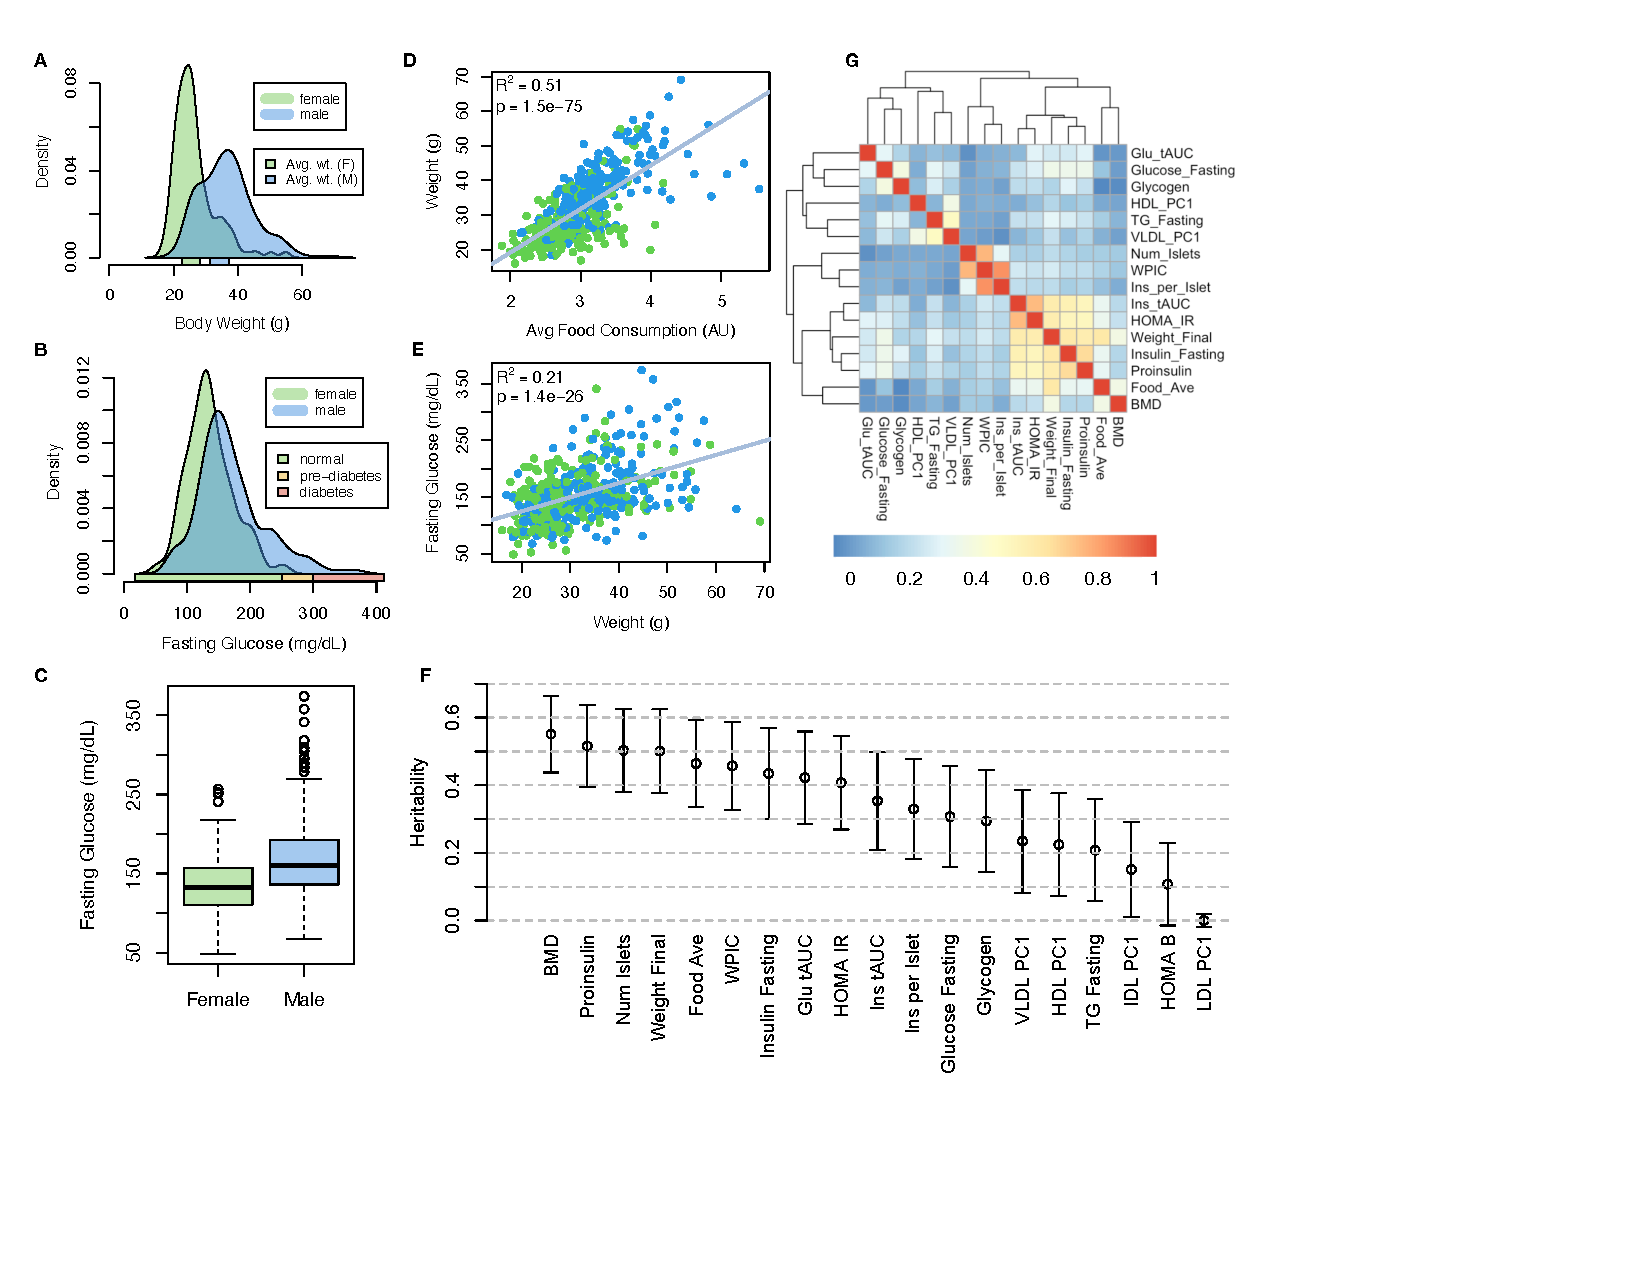
\includegraphics[width=\textwidth]{Figures/Fig1_trait_overview.pdf} 
\caption{Clinical overview. \textbf{A.} Distributions of body weight 
in the diversity outbred mice. Sex is indicated by color. The 
average B6 male and female adult weights at 24 weeks of age 
are indicated by blue and green bars on the x-axis. \textbf{B.} The 
distribution of fasting glucose across the population split 
by sex. Normal, pre-diabetic, and diabetic fasting glucose levels 
for mice are shown by colored bars along the x-axis. \textbf{C.} Males had 
higher fasting blood glucose on average than females. \textbf{D.} The 
relationship between food consumption and body weight for both 
sexes. \textbf{E.} Relationship between body weight and fasting glucose 
for both sexes. \textbf{F.} Heritability estimates for each physiological 
trait. Bars show standard error of the estimate. \textbf{G.} Correlation 
structure between pairs of physiological traits. BMD - bone mineral density,
WPIC - whole pancreas insulin content, Glu tAUC - glucose total area under 
the curve, HOMA IR - homeostatic measurement of insulin resistance, HOMA B - 
homeostatic measure of beta cell health, VLDL - very low-density lipoprotein,
LDL - low-density lipoprotein, IDL - intermediate density lipoprotein, 
HDL - high-density lipoprotein, TG - triglyceride.
}
\label{fig:trait_overview}
\end{figure}

\subsubsection{Distal Heritability Correlated with Phenotype
Relevance}\label{distal-heritability-correlated-with-phenotype-relevance}

To comprehensively assess the genetic control of gene expression in
metabolic disease we measured overall gene expression via bulk RNA-Seq
in adipose, islet, liver, and skeletal muscle in the DO cohort (Supp.
Fig. \ref{fig:eQTL}A-H). We performed eQTL analysis using R/qtl2
\cite{pmid30591514} (Methods) and identified both local and distal eQTLs
for transcripts in each of the four tissues (Supp. Fig. \ref{fig:eQTL}).
Significant local eQTLs far outnumbered distal eQTLs (Supp. Fig.
\ref{fig:eQTL}F) and tended to be shared across tissues (Supp. Fig.
\ref{fig:eQTL}G) whereas the few significant distal eQTLs we identified
tended to be tissue-specific (Supp. Fig. \ref{fig:eQTL}H)

We calculated the heritability of each transcript in terms of local and
distal genetic factors (Methods). Overall, local and distal genetic
factors contributed approximately equally to transcript abundance. In
all tissues, both local and distal factors explained between 8 and 18\%
of the variance in the median transcript (Fig, \ref{fig:motivation}A).

\begin{figure}[ht!]
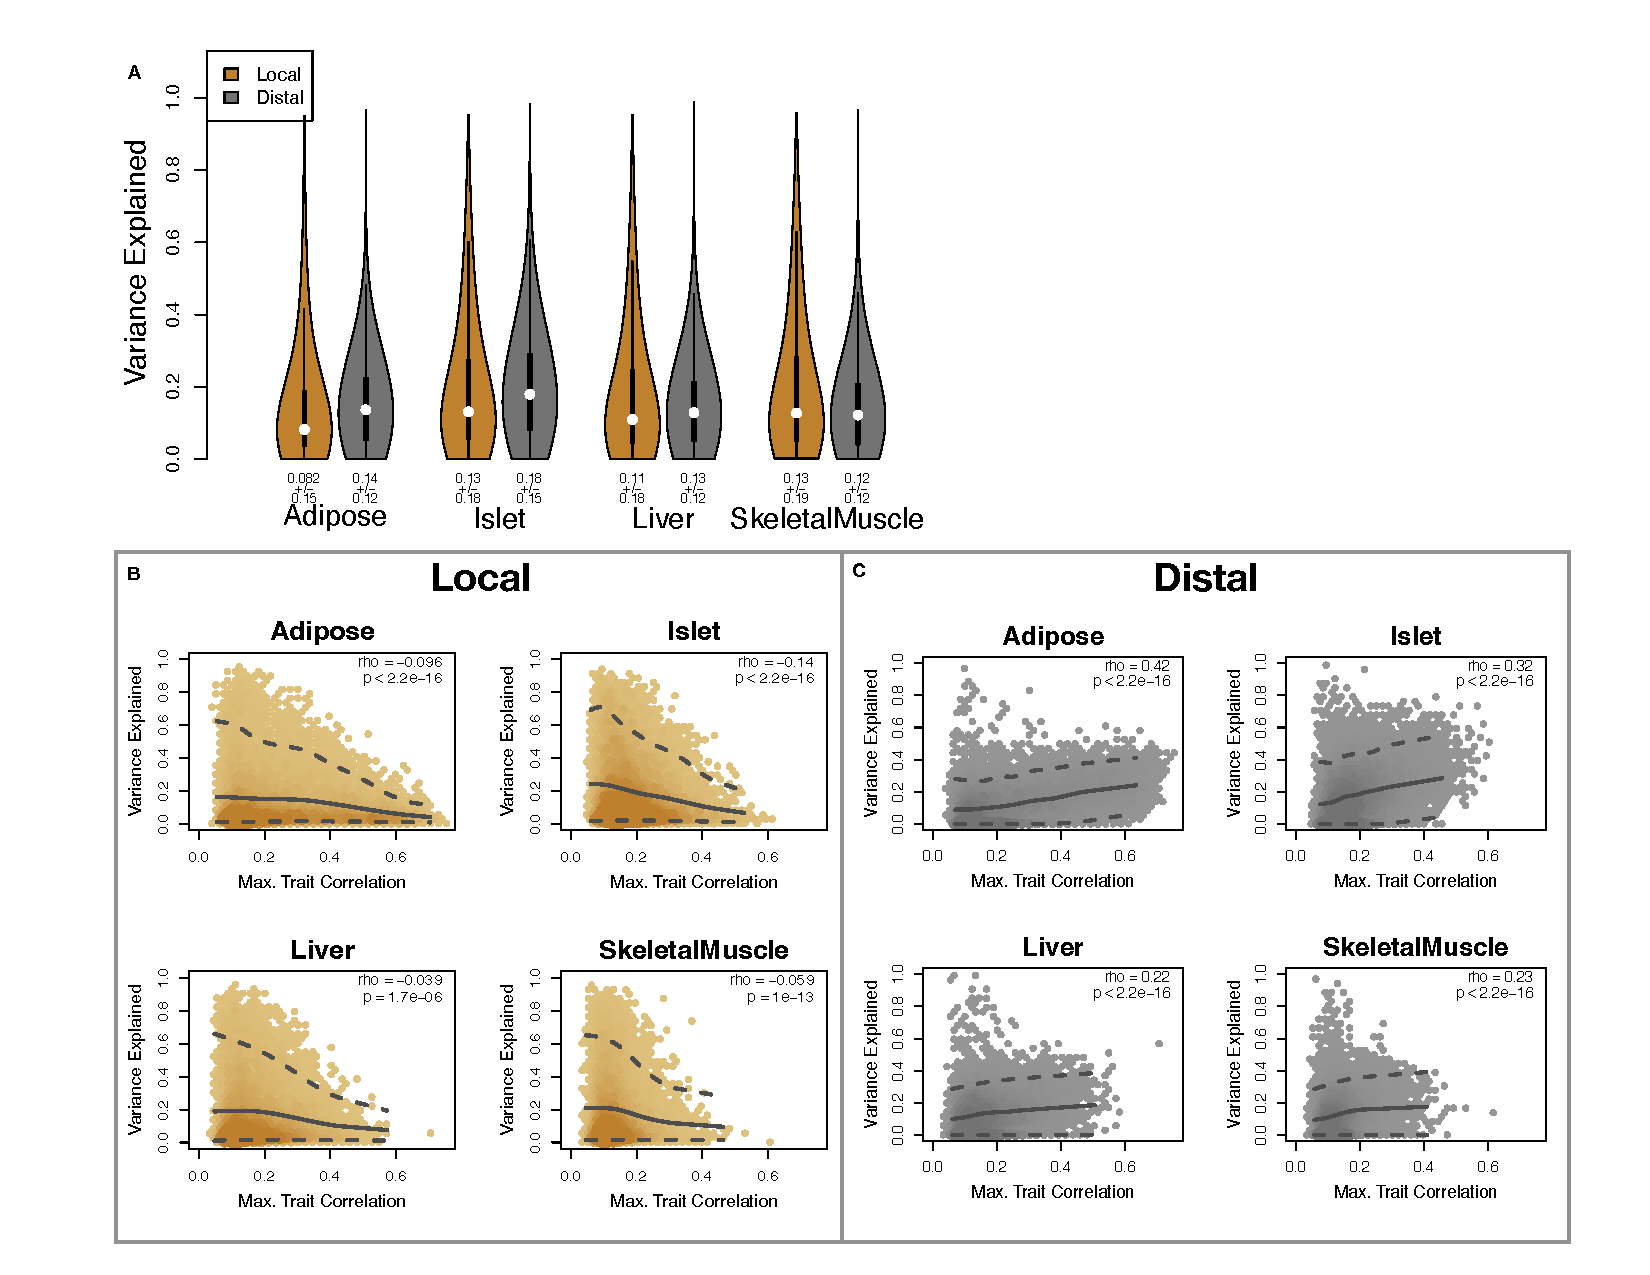
\includegraphics[width=\textwidth]{Figures/Fig2_motivation.pdf} 
\caption{Transcript heritability and trait relevance. 
\textbf{A.} Distributions of distal and local heritability of 
transcripts across the four tissues. Overall local and distal 
factors contribute equally to transcript heritability. The 
relationship between (\textbf{B.}) local and (\textbf{C.}) 
distal heritability and trait relevance across all four tissues. 
Here trait relevance is defined as the maximum correlation between 
the transcript and all traits. Local heritability was negatively 
correlated with trait relevance, and distal heritability is 
positively correlated with trait relevance. Pearson ($r$) and $p$ 
values for each correlation are shown in the upper-right of each panel.}
\label{fig:motivation}
\end{figure}

To assess the importance of genetic regulation transcript levels to
organism-level traits, we compared the local and distal heritabilities
of transcripts to their trait relevance, defined as the maximum
correlation of a transcript across all traits. The local heritability of
transcripts was negatively correlated with their trait relevance (Fig.
\ref{fig:motivation}B), suggesting that the more local genotype
influenced transcript abundance, the less effect this variation had on
the measured traits. Conversely, the distal heritability of transcripts
was positively correlated with trait relevance (Fig.
\ref{fig:motivation}C). That is, transcripts that were more highly
correlated with the measured traits tended to be distally, rather than
locally, heritable. Importantly, this pattern was consistent across all
tissues, strongly suggesting that this is a generic finding. This
finding is consistent with previous observations that low-heritability
transcripts explain more expression-mediated disease heritability than
high-heritability transcripts \cite{pmid32424349}. However, the positive
relationship between trait correlation and distal heritability
demonstrated further that there are diffuse genetic effects throughout
the genome converging on trait-related transcripts.

\subsubsection{High-Dimensional Mediation identified a high-heritability
composite trait that was mediated by a composite
transcript}\label{high-dimensional-mediation-identified-a-high-heritability-composite-trait-that-was-mediated-by-a-composite-transcript}

The above univariate analyses establish the importance of distal
heritability for trait-relevant transcripts. However, the number of
transcripts dramatically exceeds the number of phenotypes. Thus, we
expect the heritable, trait-relevant transcripts to be highly correlated
and organized according to coherent, biological processes representing
the mediating endophenotypes driving clinical trait variation. To
identify these endophenotypes in a theoretically principled way, we
developed a novel dimension-reduction technique, high-dimension
mediation analytis (HDMA), that uses the theory of causal graphical
models to identify a transcriptomic signature that is simultaneously 1)
highly heritable, 2) strongly correlated to the measured phenotypes, and
3) conforms to the causal mediation hypothesis (Fig.
\ref{fig:workflow}). HDMA projects the high-dimensional scores--a
composite genome score (\(G_C\)), a composite transcriptome score
(\(T_C\)), and a composite phenome score (\(P_C\))--and uses the
univariate theory of mediation to constrain these projections to satisfy
the hypotheses of perfect mediation, namely that upon controlling for
the transcriptomic score, the genome score is uncorrelated to the
phenome score. Formally, perfect mediation implies a constraint on the
correlation coefficients among scores as

\begin{equation*}
Corr(G_C,P_C) = Corr(G_C,T_C)Corr(T_C,P_C)
\end{equation*}

which is equivalent to the partial correlation of \(G_C\) and \(P_C\)
after controlling for \(T_C\) being zero. The value
\(Corr(G_C,T_C)Corr(T_C,P_C)\) is called the path coefficient of the
mediation model. The projections of the high-dimensional data matrices
in HDMA are designed to satisfy this constraint, and thus conform to the
perfect mediation hypothesis, as closely as possible. We stress,
however, that validating any causal assertion requires direct
experimentation and, thus, that the output of HDMA are scores that are
consistent with causal mediation. Thus, HDMA is a strategy for causal
hypothesis generation, where the causal mediator is a complex
endophenotype learned from a high-dimensional readout.

Operationally, HDMA is closely related to generalized canonical
correlation analysis (CCA), for which provably convergent algorithms
have recently been developed \cite{rgcca}. A complete mathematical
derivation and implementation details for HDMA are available in Supp.
Methods.

\begin{figure}[ht!]
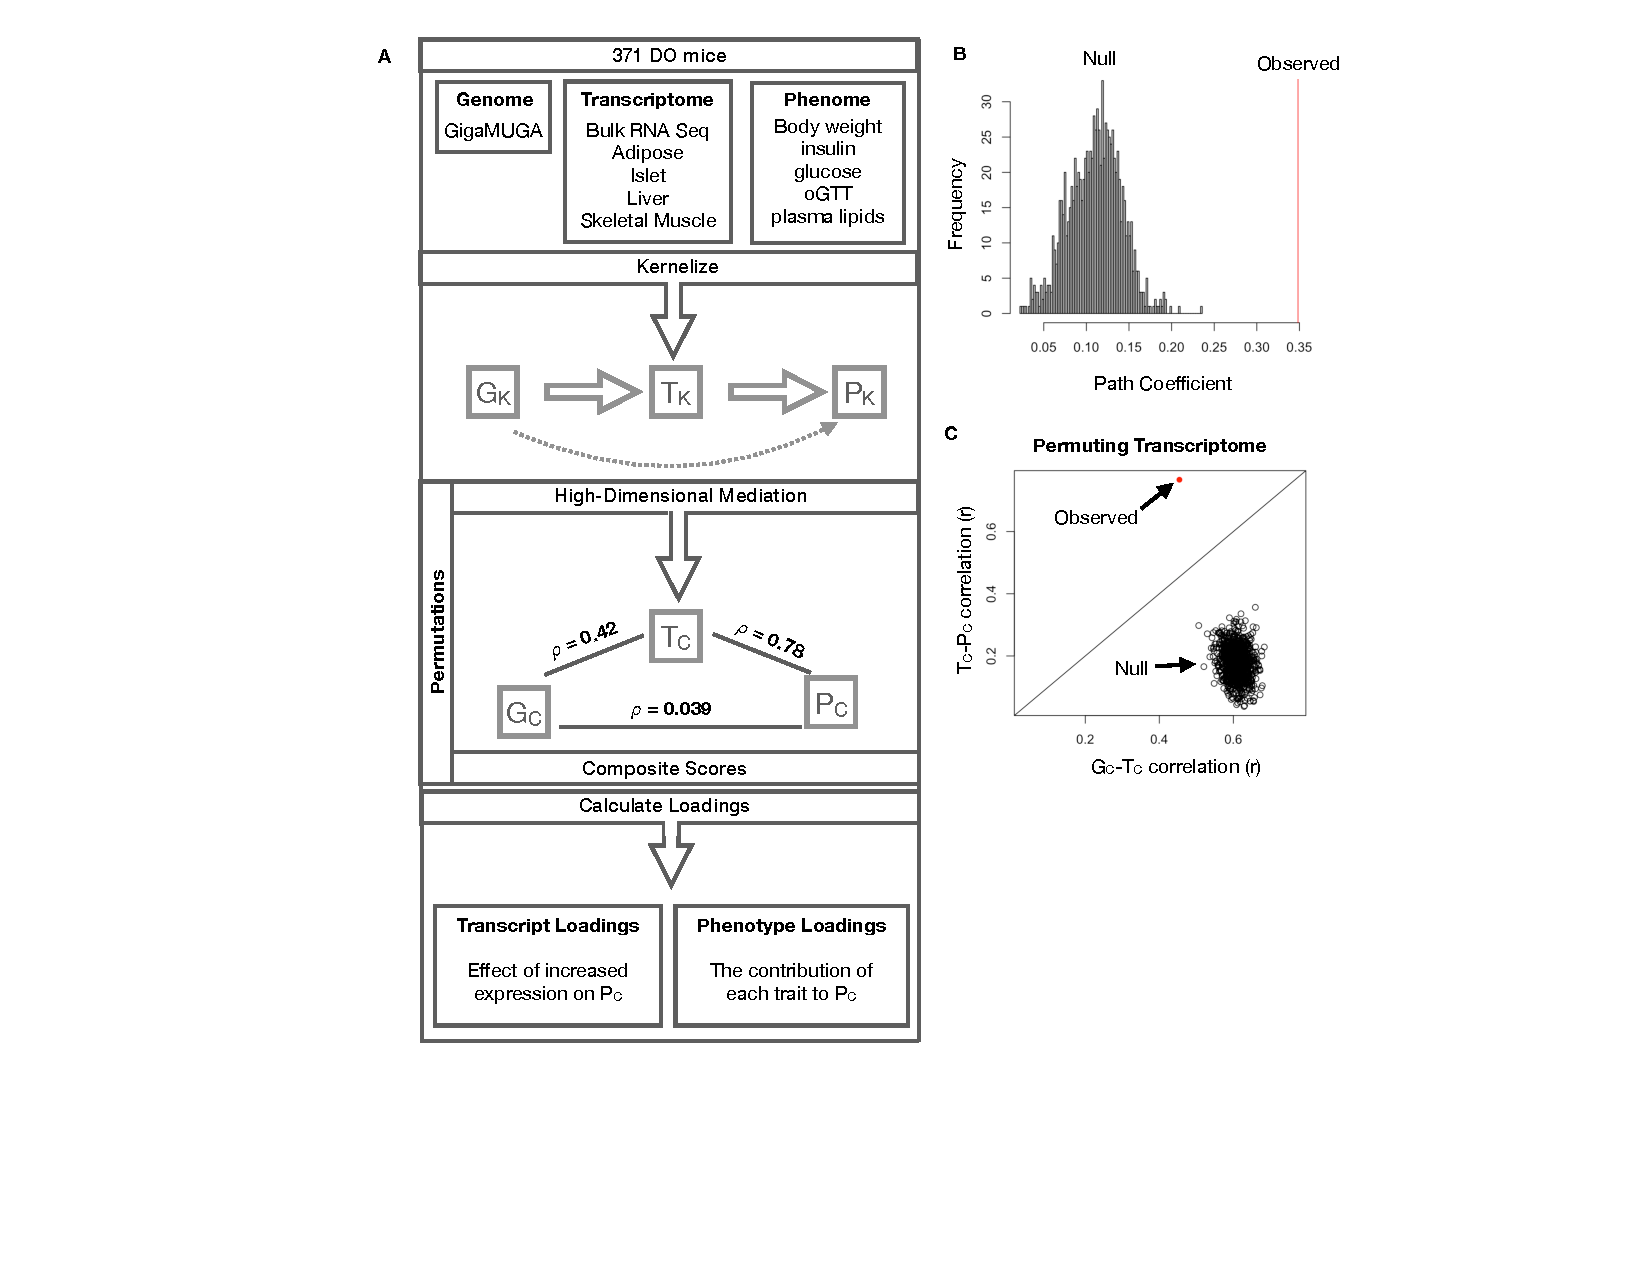
\includegraphics[width=5in]{Figures/Fig3_workflow.pdf} 
\caption{High-dimensional mediation. \textbf{A.} Workflow indicating 
major steps of high-dimensional mediation. The genotype, transcriptome, 
and phenotype matrices were independently normalized and converted to 
kernel matrices representing the pairwise relationships between 
individuals for each data modality ($K_G$ = genome kernel, $K_T$ = 
transcriptome kernel; $K_P$ = phenome kernel). 
High-dimensional mediation was applied to these matrices to maximize the 
direct path $G \rightarrow T \rightarrow P$, the mediating pathway (arrows), 
while simultaneously minimizing the direct $G \rightarrow P$ pathway (dotted 
line). The composite vectors that resulted from high-dimensional mediation were 
$G_c$, $T_C$, and $P_C$. The partial correlations $\rho$ between these vectors 
indicated perfect mediation. Transcript and trait loadings were calculated 
as described in the methods. \textbf{B.} The null distribution of the path 
coefficient derived from 10,000 permutations compared to the observed path 
coefficient (red line). \textbf{C.} The null distribution of the $G_C$-$T_C$ 
correlation vs. the $T_C$-$P_C$ correlation compared with the observed value 
(red dot).
}
\label{fig:workflow}
\end{figure}

Using HDMA we identifed the major axis of variation in the transcriptome
that was consistent with mediating the effects of the genome on
metabolic traits (Fig \ref{fig:workflow}). Fig. \ref{fig:workflow}A
shows the partial correlations (\(\rho\)) between the pairs of these
composite vectors. The partial correlation between \(G_C\) and \(T_C\)
was 0.42, and the partial correlation between \(T_C\) and \(P_C\) was
0.78. However, when the transcriptome was taken into account, the
partial correlation between \(G_C\) and \(P_C\) was effectively zero
(0.039). \(P_C\) captured 30\% of the overall trait variance, and its
estimated heritability was 0.71 \(\pm\) 0.084, which was higher than any
of the measured traits (Fig. \ref{fig:trait_overview}F). Thus, HDMA
identified a maximally heritable metabolic composite trait and a highly
heritable component of the transcriptome that are correlated as expected
in the perfectly mediated model.

As discussed in Supp. Methods, HDMA is related to a generalized form of
CCA. Standard CCA is prone to over-fitting because in any two large
matrices it can be trivial to identify highly correlated composite
vectors \cite{pmid38383808}. To assess whether our implementation of
HDMA was similarly prone to over-fitting in a high-dimensional space, we
performed permutation testing. We permuted the individual labels on the
transcriptome matrix 1000 times and recalculated the path coefficient,
which is the partial correlation of \(G_C\) and \(T_C\) multiplied by
the partial correlation of \(T_C\) and \(P_C\). This represents the
strength of the path from \(G_C\) to \(P_C\) that is putatively mediated
through \(T_C\). The null distribution of the path coefficient is shown
in Fig. \ref{fig:workflow}B, and the observed path coefficient from the
original data is indicated by a red line. The observed path coefficient
was well outside the null distribution generated by permutations
(\(p < 10^{-16}\)). Fig. \ref{fig:workflow}C illustrates this
observation in more detail. Although we identified high correlations
between \(G_C\) and \(T_C\), and modest correlations between \(T_C\) and
\(P_C\) in the null data (Fig \ref{fig:workflow}C), these two values
could not be maximized simultaneously in the null data. In contrast, the
red dot shows that in the real data both the \(G_C\)-\(T_C\) correlation
and the \(T_C\)-\(P_C\) correlation could be maximized simultaneously
suggesting that the path from genotype to phenotype through
transcriptome is highly non-trivial and identifiable in this case. These
results suggest that these composite vectors represent genetically
determined variation in phenotype that is mediated through genetically
determined variation in transcription.

\subsubsection{Body weight and insulin resistance were highly
represented in the expression-mediated composite
trait}\label{body-weight-and-insulin-resistance-were-highly-represented-in-the-expression-mediated-composite-trait}

Each composite score is simply a weighted combination of the measured
variables and the magnitude and sign of the weights, called loadings,
correspond the relative importance and directionality of each variable
in the composite score. The loadings of each measured trait onto \(P_C\)
indicate how much each contributed to the composite phenotype. Body
weight contributed the most (Fig. \ref{fig:interpretation}), followed by
homeostatic insulin resistance (HOMA\_IR) and fasting plasma insulin
levels (Insulin\_Fasting). We can thus interpret \(P_C\) as an index of
metabolic disease (Fig. \ref{fig:interpretation}B). Individuals with
high values of \(P_C\) have a higher metabolic disease index and greater
metabolic disease, including higher body weight and higher insulin
resistance. We refer to \(P_C\) as the metabolic disease index (MDI)
going forward. Traits contributing the least to the MDI were measures of
cholesterol and pancreas composition. Thus, when we interpret the
transcriptomic signature identified by HDMA, we are explaining primarily
the putative transcriptional mediation of body weight and insulin
resistance, as opposed to cholesterol measurements.

\begin{figure}[ht!]
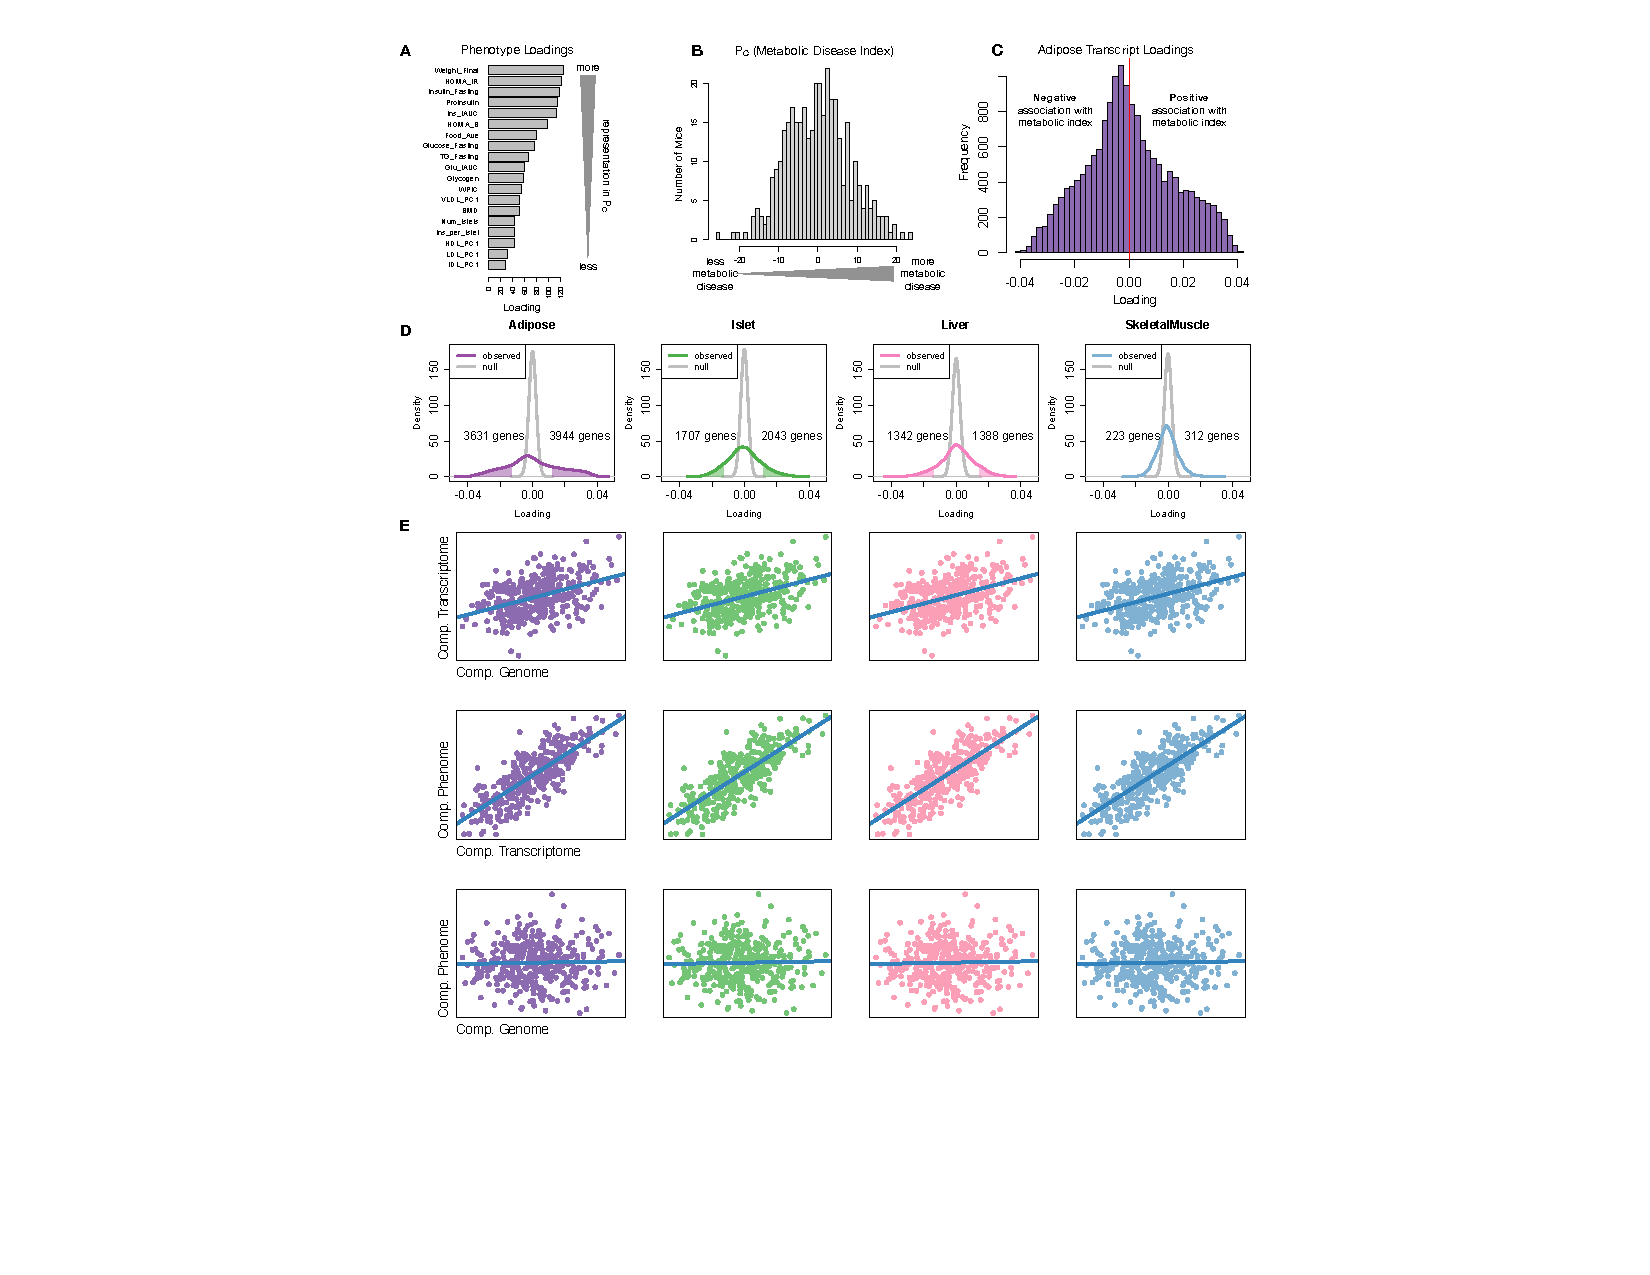
\includegraphics[width=\textwidth]{Figures/Fig4_interpretation.pdf} 
\caption{Interpretation of loadings. \textbf{A.} Loadings 
across traits. Body weight and insulin resistance contributed 
the most to the composite trait. \textbf{B.} Phenotype scores 
across individuals. Individuals with large positive phenotype 
scores had higher body weight and insulin resistance than average. 
Individuals with large negative phenotype scores had lower body 
weight and insulin resistance than average. \textbf{C.} 
Distribution of transcript loadings in adipose tissue. For 
transcripts with large positive loadings, higher expression was 
associated with higher phenotype scores. For transcripts with 
large negative loadings, higher expression was associated with 
lower phenotype scores. \textbf{D.} Distribution of absolute 
value of transcript loadings across tissues. Transcripts in 
adipose tissue had the largest loadings indicating that 
adipose tissue gene expression was a strong mediator of 
genotype on body weight and insulin resistance.
}
\label{fig:interpretation}
\end{figure}

\subsubsection{High-loading transcripts have low local heritability,
high distal heritability, and were linked mechanistically to
obesity}\label{high-loading-transcripts-have-low-local-heritability-high-distal-heritability-and-were-linked-mechanistically-to-obesity}

We interpreted large loadings onto transcripts as indicating strong
mediation of the effect of genetics on MDI. Large positive loadings
indicate that higher expression was associated with a higher MDI
(i.e.~higher risk of obesity and metabolic disease on the HFHS diet)
(Fig. \ref{fig:interpretation}C). Conversely, large negative loadings
indicate that high expression of these transcripts was associated with a
lower MDI (i.e.~lower risk of obesity and metabolic disease on the HFHS
diet) (Fig. \ref{fig:interpretation}C). We used gene set enrichment
analysis (GSEA) \cite{fgsea, 
pmid16199517} to look for biological processes and pathways that were
enriched at the top and bottom of this list (Methods).

In adipose tissue, both GO processes and KEGG pathway enrichments
pointed to an axis of inflammation and metabolism (Figs.
\ref{fig:top_enrich_kegg} and \ref{fig:top_enrich_go}). GO terms and
KEGG pathways associated with inflammation were positively associated
with MDI, indicating that increased expression in inflammatory pathways
was associated with a higher MDI. It is well established that adipose
tissue in obese individuals is inflamed and infiltrated by macrophages
\cite{pmid19133410, 
pmid28955384, pmid28912810, pmid28901330, pmid24969772}, and the results
here suggest that this may be a dominant heritable component of
metabolic disease.

The strongest negative enrichments in adipose tissue were related to
mitochondial activity in general, and thermogenesis in particular (Figs.
\ref{fig:top_enrich_kegg} and \ref{fig:top_enrich_kegg}). Genes in the
KEGG oxidative phosphorylation pathway in mice were almost universally
negatively loaded in adipose tissue, suggesting that increased
expression of these genes was associated with reduced MDI (Supp. Fig.
\ref{fig:oxPhos}). Consistent with this observations, it has been shown
previously that mouse strains with greater thermogenic potential are
also less susceptible to obesity on a HFHS diet \cite{pmid18492779}.

Transcripts associated with the citric acid (TCA) cycle as well as the
catabolism of the branched-chain amino acids (BCAA) (valine, leuceine,
and isoleucine) were strongly enriched with negative loadings in adipose
tissue (Supp. Figs. \ref{fig:top_enrich_kegg}, \ref{fig:TCA_cycle} and
\ref{fig:bcaa_degrataion}). Expression of genes in both pathways (for
which there is some overlap) has been previously associated with insulin
sensitivity \cite{pmid29567659, 
pmid22560213, pmid19841271}, suggesting that heritable variation in
regulation of these pathways may influence risk of insulin resistance.

Looking a the 10 most positively and negatively loaded transcripts from
each tissue, it is apparent that transcripts in the adipose tissue had
the largest loadings, both positive and negative, of all tissues (Fig.
\ref{fig:loading_heritability}A bar plot) This suggests that much of the
effect of genetics on body weight and insulin reisistance is mediated
through gene expression in adipose tissue. The strongest loadings in
liver and pancreas were comparable, and those in skeletal muscle were
the weakest (Fig. \ref{fig:loading_heritability}A), suggesting that less
of the genetic effects were mediated through transcription in skeletal
muscle. Heritability analysis showed that transcripts with the largest
loadings had higher distal heritability than local heritability (Fig.
\ref{fig:loading_heritability}A heat map and box plot). This pattern
contrasts with transcripts nominated by TWAS (Fig.
\ref{fig:loading_heritability}B), which tended to have lower loadings,
higher local heritability and lower distal heritability. Transcripts
with the highest local heritability in each tissue (Fig.
\ref{fig:loading_heritability}C) had the lowest loadings, consistent
with our findings above (Fig. \ref{fig:motivation}B).

We performed a literature search for the genes in each of these groups
along with the terms ``diabetes'', ``obesity'', and the name of the
expressing tissue to determine whether any of these genes had previous
associations with metabolic disease in the literature (Methods).
Multiple genes in each group had been previously associated with obesity
and diabetes (Fig. \ref{fig:loading_heritability} bolded gene names).
Genes with high loadings were most highly enriched for previous
literature support. They were 2.4 times more likely than TWAS hits and
3.8 times more likely than genes with high local heritability to be
previously associated with obesity or diabetes.

\begin{figure}[ht!]
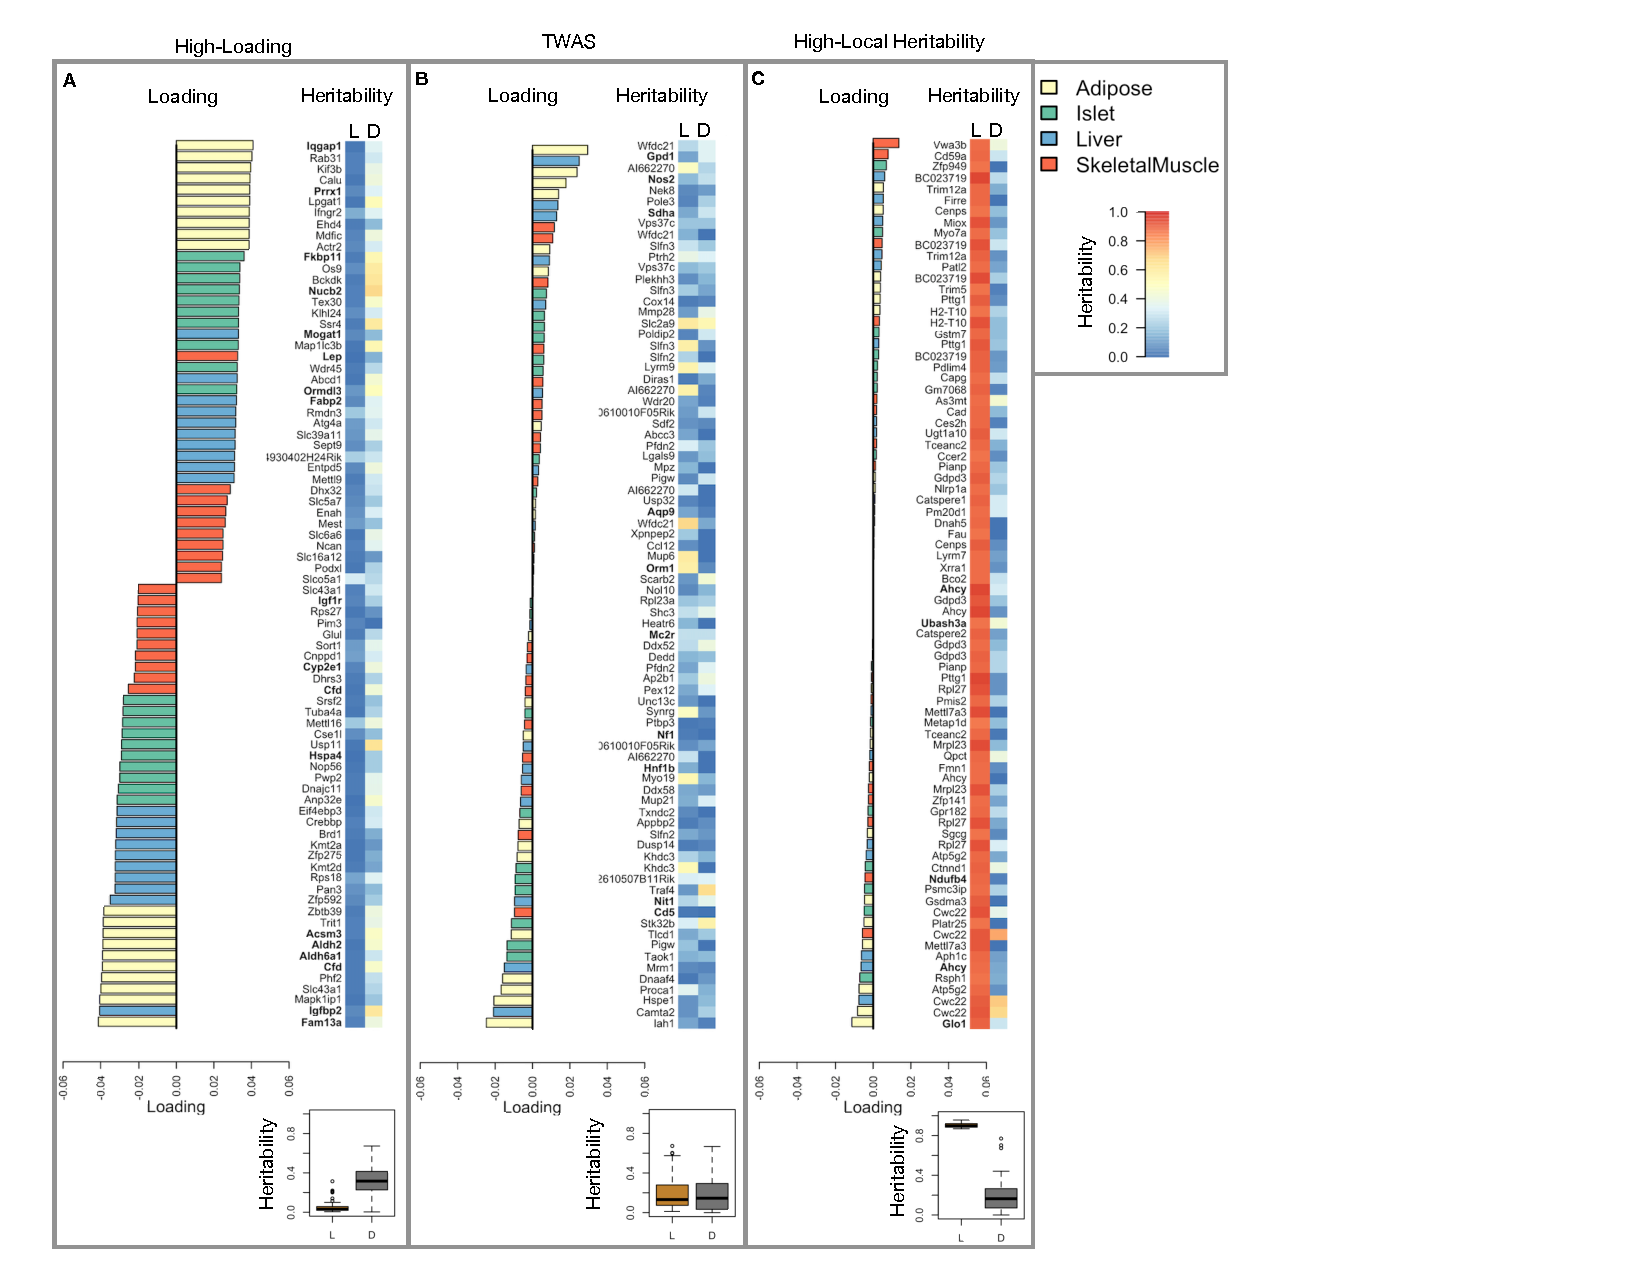
\includegraphics[width=\textwidth]{Figures/Fig5_loading_heritability.pdf} 
\caption{Transcripts with high loadings have high distal heritability
and literature support. Each panel has a bar plot showing the loadings 
of transcripts selected by different criteria. Bar color indicates the 
tissue of origin. The heat map shows the local (L - left) and distal 
(D - right) heritability of each transcript. \textbf{A.} Loadings for 
the 10 transcripts with the largest positive loadings and the 10 
transcripts with the largest negative loadings for each tissue. 
\textbf{B.} Loadings of TWAS candidates with the 10 largest positive 
correlations with traits and the largest negative correlations with 
traits across all four tissues. \textbf{C.} The transcripts with the 
largest local heritability (top 20) across all four tissues.
}
\label{fig:loading_heritability}
\end{figure}

\subsubsection{Tissue-specific transriptional programs were associated
with metabolic
traits}\label{tissue-specific-transriptional-programs-were-associated-with-metabolic-traits}

Clustering of transcripts with top loadings in each tissue showed
tissue-specific functional modules associated with obesity and insulin
resistance (Fig. \ref{fig:toa}A) (Methods). The clustering highlights
the importance of immune activation particularly in adipose tissue. The
``mitosis'' cluster had large positive loadings in three of the four
tissues potentially suggesting system-wide proliferation of immune
cells. Otherwise, all clusters were strongly loaded in only one or two
tissues. For example, the lipid metabolism cluster was loaded most
heavily in liver. The positive loadings suggest that high expression of
these genes particularly in the liver was associated with increased
metabolic disease. This cluster included the gene \textit{Pparg}, whose
primary role is in the adipose tissue where it is considered a master
regulator of adipogenesis \cite{pmid17389767}. Agonists of
\textit{Pparg}, such as thiazolidinediones, are FDA-approved to treat
type II diabetes, and reduce inflammation and adipose hyptertrophy
\cite{pmid17389767}. Consistent with this role, the loading for
\textit{Pparg} in adipose tissue was negative, suggesting that higher
expression was associated with leaner mice (Fig. \ref{fig:toa}B). In
contrast, \textit{Pparg} had a large positive loading in liver, where it
is known to play a role in the development of hepatic steatosis, or
fatty liver. Mice that lack \textit{Pparg} specifically in the liver,
are protected from developing steatosis and show reduced expression of
lipogenic genes \cite{pmid12805374, pmid12618528}. Overexpression of
\textit{Pparg} in the livers of mice with a \textit{Ppara} knockout,
causes upregulation of genes involved in adipogenesis
\cite{pmid16357043}. In the livers of both mice and humans high
\textit{Pparg} expression is associated with hepatocytes that accumulate
large lipid droplets and have gene expression profiles similar to that
of adipocytes \cite{pmid15644454, pmid16403437}.

The local and distal heritability of \textit{Pparg} is low in adipose
tissue suggesting its expression in this tissue is highly constrained in
the population (Fig. \ref{fig:toa}B). However, the distal heritability
of \textit{Pparg} in liver is relatively high suggesting it is complexly
regulated and has sufficient variation in this population to drive
variation in phenotype. Both local and distal heribatility of
\textit{Pparg} in the islet are relatively high, but the loading is low,
suggesting that variability of expression in the islet does not drive
variation in MDI. These results highlight the importance of tissue
context when investigating the role of heritable transcript variability
in driving phenotype.

Gene lists for all clusters are available in Supp. File 1.

\begin{figure}[ht!]
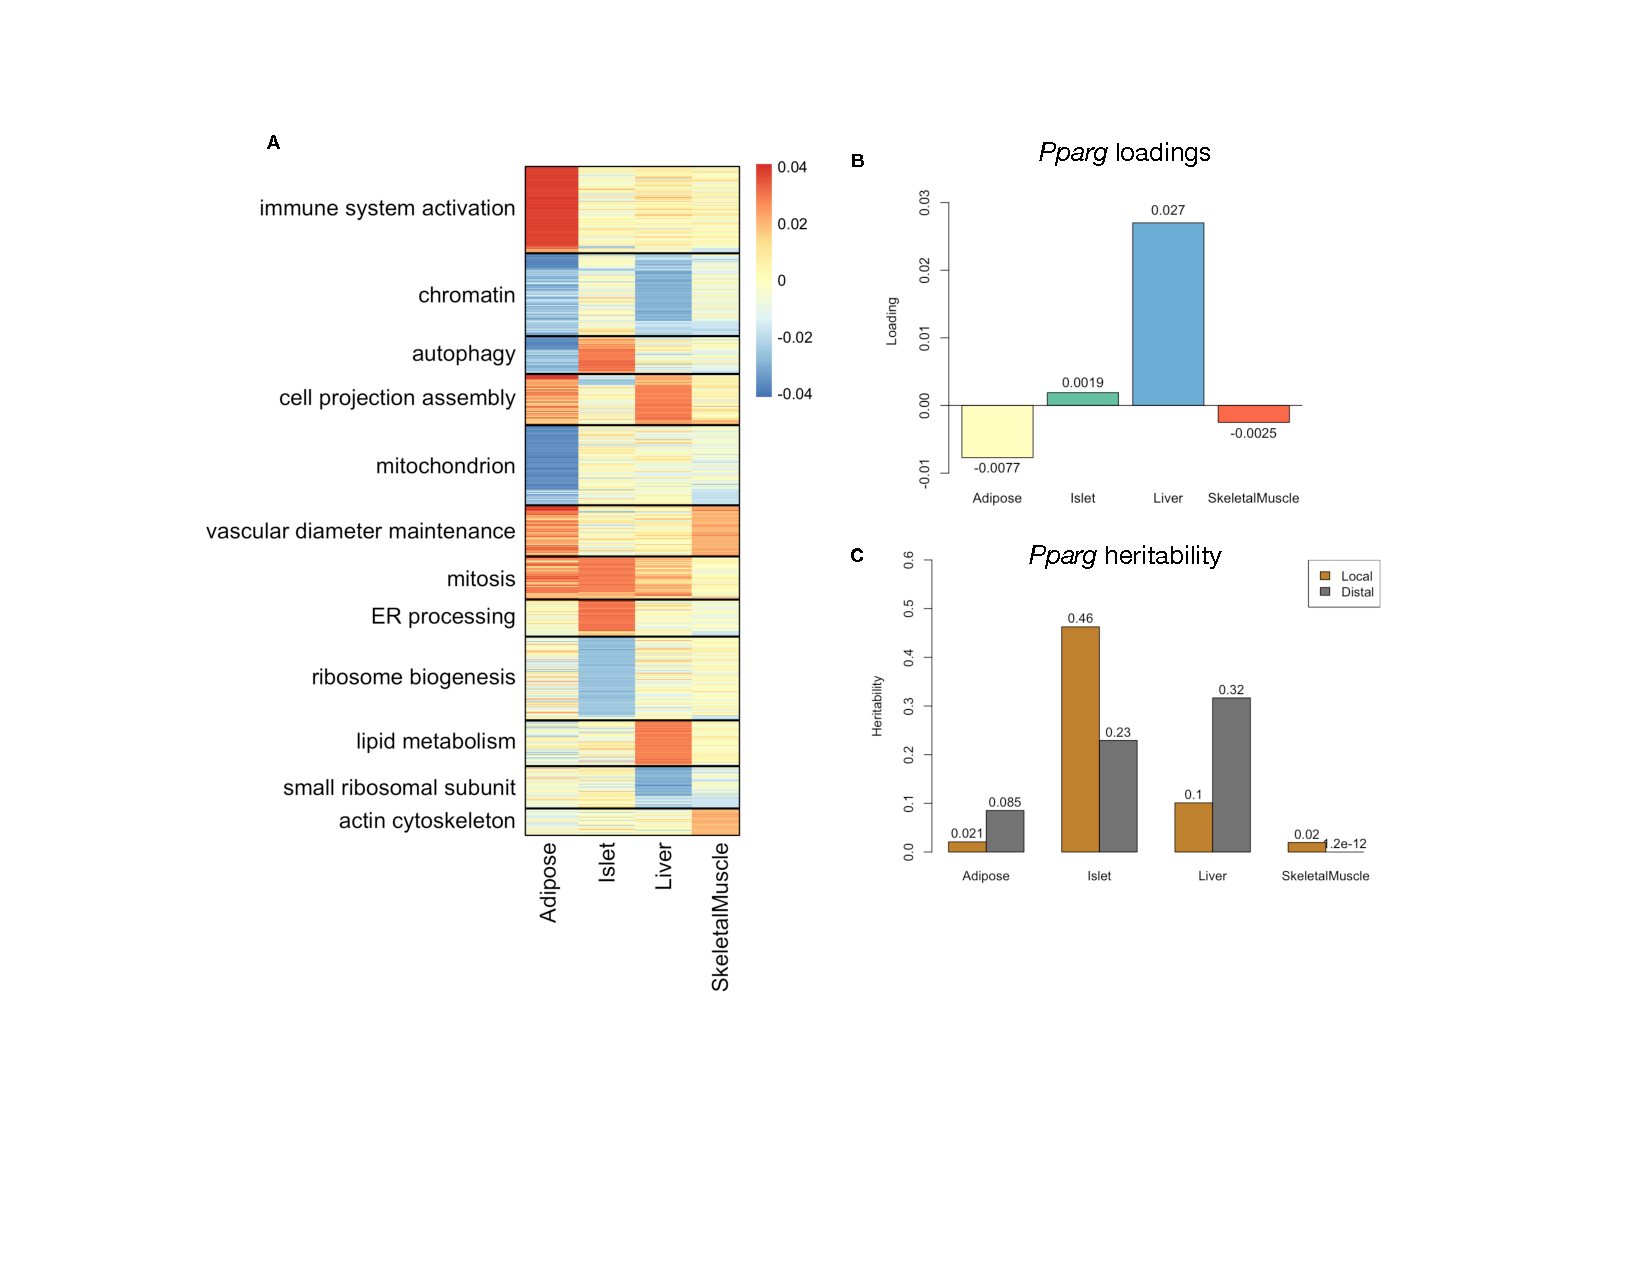
\includegraphics[width=\textwidth]{Figures/Fig6_TOA.pdf} 
\caption{Tissue-specific transcriptional programs were associated 
with obesity and insulin resistance. \textbf{A} Heat map showing 
the loadings of all transcripts with loadings greater than 2.5 
standard deviations from the mean in any tissue. The heat map was 
clustered using k medoid clustering. Functional enrichments of each 
cluster are indicated along the left margin. \textbf{B} Loadings for 
\textit{Pparg} in different tissues. \textbf{C} Local and distal of 
\textit{Pparg} expression in different tissues.
}
\label{fig:toa}
\end{figure}

\subsubsection{Gene expression, but not local eQTLs, predicted body
weight in an independent
population}\label{gene-expression-but-not-local-eqtls-predicted-body-weight-in-an-independent-population}

To test whether the transcript loadings identified in the DO could be
translated to another population, we tested whether they could predict
metabolic phenotype in an independent population of CC-RIX mice, which
were F1 mice derived from multiple pairings of Collaborative Cross (CC)
\cite{pmid28592495, pmid21411855, 
pmid17674098, pmid15514660} strains (Fig. \ref{fig:cc_prediction})
(Methods). We tested two questions. First, we asked whether the loadings
identified in the DO mice were relevant to the relationship between the
transcriptome and the phenome in the CC-RIX. We predicted body weight (a
surrogate for MDI) in each CC-RIX individual using measured gene
expression in each tissue and the transcript loadings identified in the
DO (Methods). The predicted body weight and acutal body weight were
highly correlated in all tissues (Fig. \ref{fig:cc_prediction}B left
column). The best prediction was achieved for adipose tissue, which
supports the observation in the DO that adipose expression was the
strongest mediator of the genetic effect on MDI. This result also
confirms the validity and translatability of the transcript loadings and
their relationship to metabolic disease.

\begin{figure}[ht!]
\includegraphics[width=\textwidth]{Figures/Fig7_CC_Prediction.pdf} 
\caption{Transcription, but not local genotype, predicts 
phenotype in the CC-RIX. \textbf{A.} Workflow showing procedure 
for translating HDMA results to an independent population of mice. 
\textbf{B.} Relationships between the predicted metabolic disease
index (MDI) and measured body weight. The left column shows the 
predictions using measured transcripts. The right column shows 
the prediction using transcript levels imputed from local genotype. 
Gray boxes indicate measured quantities, and blue boxes indicate 
calculated quantities. The dots in each panel represent individual 
CC-RIX strains. The gray lines show the standard deviation on body 
weight for the strain.
}
\label{fig:cc_prediction}
\end{figure}

The second question related to the source of the relevant variation in
gene expression. If local regulation was the predominant factor
influencing gene expression, we should be able to predict phenotype in
the CC-RIX using transcripts imputed from local genotype (Fig.
\ref{fig:cc_prediction}A). The DO and the CC-RIX were derived from the
same eight founder strains and so carry the same alleles throughout the
genome. We imputed gene expression in the CC-RIX using local genotype
and were able to estimate variation in gene transcription robustly
(Supp. Fig. \ref{fig:cc_imputation}). However, these imputed values
failed to predict body weight in the CC-RIX when weighted with the
loadings from HDMA. (Fig. \ref{fig:cc_prediction}B right column). This
result suggests that local regulation of gene expression is not the
primary factor driving heritability of complex traits, consistent with
our findings in the DO population that distal heritability was a major
driver of trait-relevant variation and that high-loading transcripts had
comparatively high distal and low local heritability.

\subsubsection{Distally heritable transcriptomic signatures reflected
variation in composition of adipose tissue and
islets}\label{distally-heritable-transcriptomic-signatures-reflected-variation-in-composition-of-adipose-tissue-and-islets}

The interpretation of global genetic influences on gene expression and
phenotype is potentially more challenging than the interpretation and
translation of local genetic influences, as genetic effects cannot be
localized to individual gene variants or transcripts. However, there are
global patterns across the loadings that can inform mechanism. For
example, heritable variation in cell type composition can be inferred
from transcript loadings. We observed above that immune activation in
the adipose tissues was a highly enriched process correlating with
obesity in the DO population. For example, in humans, it has been
extensively observed that macrophage infiltration in adipose tissue is a
marker of obesity and metabolic disease \cite{pmid24781408}. To
determine whether the immune activation reflected a heritable change in
cell composition in adipose tissue in DO mice, we compared loadings of
cell-type specific genes in adipose tissue (Methods). Consistent with
human results, the mean loading of macrophage-specific genes was
significantly greater than 0 (Fig. \ref{fig:human_translation}A),
indicating that obese mice were genetically predisposed to have high
levels of macrophage infiltration in adipose tissue in response to the
HFHS diet. Loading for marker genes for other cell types were not
statistically different from zero, indicating that changes in the
abundance of those cell types is not a mediator of MDI.

\begin{figure}[ht!]
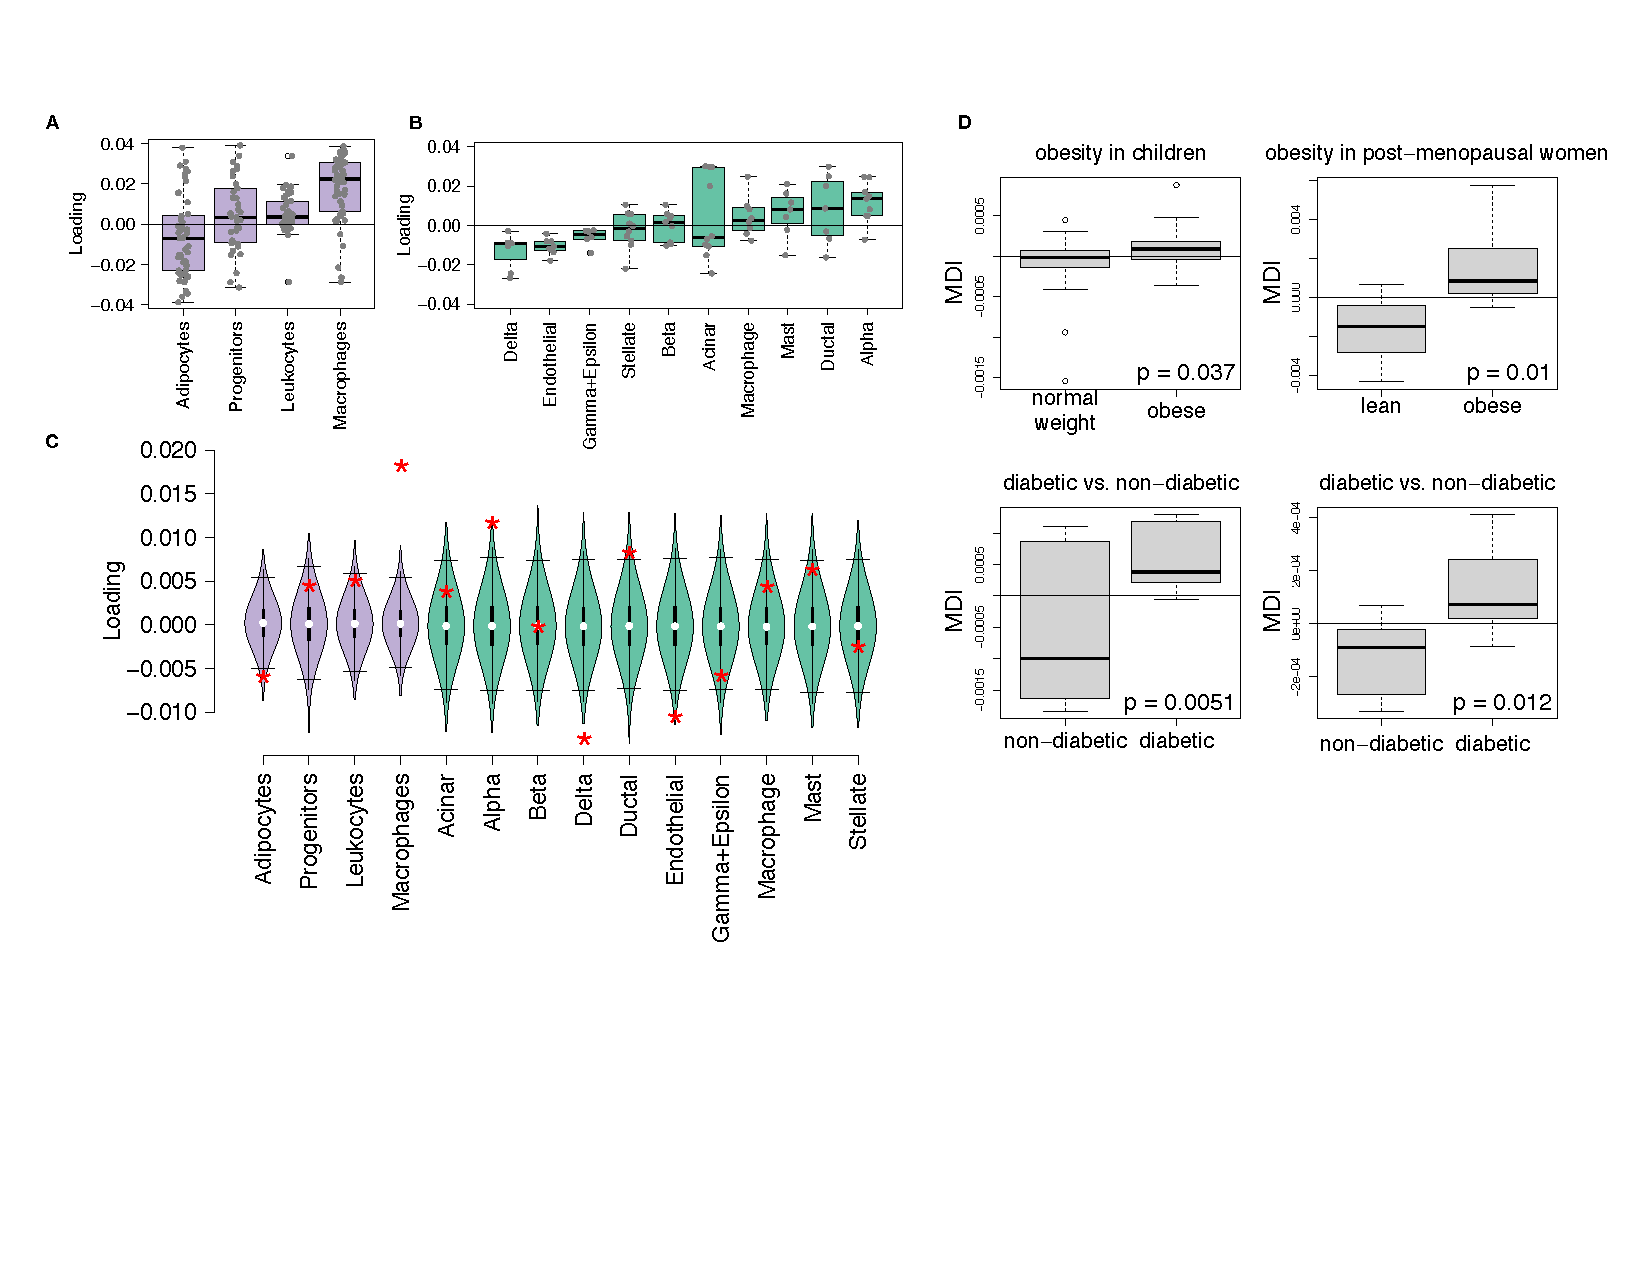
\includegraphics[width=\textwidth]{Figures/Fig8_Human_Translation.pdf} 
\caption{HDMA results translate to humans. \textbf{A.} Distribution of 
loadings for cell-type-specific transcripts in adipose tissue. \textbf{B.} 
Distribution of loadings for cell-type-specific transcripts in pancreatic 
islets (green). \textbf{C.} Null distributions for the mean loading of 
randomly selected transcripts in each cell type compared with the observed 
mean loading of each group of transcripts (red asterisk). \textbf{D.} 
Predictions of metabolic phenotypes in four adipose transcription data 
sets downloaded from GEO. In each study the obese/diabetic patients were 
predicted to have greater metabolic disease than the lean/non-diabetic 
patients based on the HDMA results from DO mice.
}
\label{fig:human_translation}
\end{figure}

We also compared loadings of cell-type specific transcripts in islet
(Methods). The mean loadings for alpha-cell specific transcripts were
significantly greater than 0, while the mean loadings for delta- and
endothelial-cell specific genes were significantly less than 0 (Fig.
\ref{fig:human_translation}B). These results suggest either that mice
with higher MDI had inherited a higher proportions of alpha cells, and
lower proportions of endothelial and delta cells in their pancreatic
islets, that such compositional changes were induced by the HFHS diet in
a heritable way, or both. In either case, these results support the
hypothesis that alterations in islet composition drive variation in MDI.

Notably, the loadings for pancreatic beta cell-type specific loadings
was not significantly different from zero. We stress that this is not
necessarily reflective of the function of the beta cells in the obese
mice, but rather suggests that any variation in the number of beta cells
in these mice was unrelated to obesity and insulin resistance, the major
contributors to MDI. This is further consistent with the islet
composition traits having small loadings in the phenome score (Fig.
\ref{fig:interpretation}).

\subsubsection{Heritable transcriptomic signatures translated to human
disease}\label{heritable-transcriptomic-signatures-translated-to-human-disease}

Ultimately, the heritable transcriptomic signatures that we identified
in DO mice will be useful if they inform pathogenicity and treatment of
human disease. To investigate the potential for translation of the gene
signatures identified in DO mice, we compared them to transcriptional
profiles in obese and non-obese human subjects (Methods). We limited our
analysis to adipose tissue because the adipose tissue signature had the
strongest relationship to obesity and insulin resistance in the DO.

We calculated a predicted obesity score for each individual in the human
studies based on their adipose tissue gene expression (Methods) and
compared the predicted scores for obese and non-obese groups as well as
diabetic and non-diabetic groups. In all cases, the predicted obesity
scores were higher on average for individuals in the obese and diabetic
groups compared with the lean and non-diabetic groups (Fig.
\ref{fig:human_translation}D). This indicates that the distally
heritable signature of MDI identified in DO mice is relevant to obesity
and diabetes in human subjects.

\subsubsection{Existing therapies are predicted to target mediator gene
signatures}\label{existing-therapies-are-predicted-to-target-mediator-gene-signatures}

Another potential application of the transcript loading landscape is in
ranking potential drug candidates for the treatment of metabolic
disease. Although high-loading transcripts may be good candidates for
understanding specific biology related to obesity, the transcriptome
overall is highly interconnected and redundant. The ConnectivityMap
(CMAP) database \cite{pmid17008526} developed by the Broad Institute
allows querying thousands of compounds that reverse or enhance the
extreme ends of transcriptomic signatures in multiple different cell
types. By identifying drugs that reverse pathogenic transcriptomic
signatures, we can potentially identify compounds that have favorable
effects on gene expression.

To test this hypothesis, we queried the CMAP database through the CLUE
online query tool (\url{https://clue.io/query/}, version 1.1.1.43)
(Methods). We identified top anti-correlated hits across all cell types
(Supp. Figs \ref{fig:clue_adipose_all} and \ref{fig:clue_islet_all}). To
get more tissue-specific results, we also looked at top results in cell
types that most closely resembled our tissues. We looked at results in
adipocytes (ASC) as well as pancreatic tumor cells (YAPC) regardless of
\(p\) value (Supp. Figs \ref{fig:clue_adipose_asc} and
\ref{fig:clue_islet_yapc}).

Looking across all cell types, the notable top hits from the adipose
tissue loadings included mTOR inhibitors and glucocorticoid agonists
(Supp. Fig. \ref{fig:clue_adipose_all}). It is thought that metformin,
which is commonly used to improve glycemic control, acts, at least in
part, by inhibiting mTOR signaling \cite{pmid30290005, 
pmid30034573}. However, long-term use of other mTOR inhibitors, such as
rapamycin, are known to cause insulin resistance and \(\beta\)-cell
toxicity \cite{pmid30034573, pmid23881200, pmid21266327}.
Glucocorticoids are used to reduce inflammation, which was a prominent
signature in the adipose tissues, but these drugs also promote
hyperglycemia and diabetes \cite{pmid24582093, pmid35585199}. Accute
treatment with glucocorticoids has further been shown to reduce
thermogenesis in rodent adipocytes \cite{pmid30310815, 
pmid11254472, pmid23197361}, but increase thermogenesis in human
adipocytes \cite{pmid27411014, pmid25385872}. Thus, the pathways
identified by CMAP across all cell types were highly related to the
transcript loading profiles, but the relationship was not a simple
reversal.

The top hit for the adipose composite transcript in CMAP adipocytes was
a PARP inhibitor (Supp. Fig. \ref{fig:clue_adipose_asc}). PARPs play a
role in lipid metabolism and are involved in the development of obesity
and diabetes \cite{pmid34450194}. PARP1 inhibition increases
mitochondrial biogenesis \cite{pmid21459330}. Inihibition of PARP1
activity can further prevent necrosis in favor of the less inflammatory
apoptosis \cite{pmid12114611}, thereby potentially reducing inflammation
in stressed adipocytes. Other notable hits among the top 20 were BTK
inhibitors, which have been observed to suppress inflammation and
improve insulin resistance \cite{pmid33648925} as well as to reduce
insulin antibodies in type I diabetes \cite{pmid28753229}. IkappaB
kinase (IKK) is an enzyme complex involved in regulating cellular
responses to inflammation \cite{pmid17047224}. Inhibitors of IKK have
been shown to improve glucose control in type II diabetes
\cite{pmid28683283, 
pmid15685170}.

Among the top most significant hits for the transcript loadings from
pancreatic islets (Supp. Fig. \ref{fig:clue_islet_all}), was suppression
of T cell receptor signaling, which is known to be involved in Type 1
diabetes \cite{pmid33603744}, as well as TNFR1, which has been
associated with mortality in diabetes patients \cite{pmid32281000}.
Suppression of NOD1/2 signaling was also among the top hits. NOD1 and 2
sense ER stress \cite{pmid27007849, pmid28823510}, which is associated
with \(\beta\)-cell death in type 1 and type 2 diabetes
\cite{pmid24520198}. This cell death process is dependent on NOD1/2
signaling \cite{pmid27007849}, although the specifics have not yet been
worked out.

We also looked specifically at hits in pancreatic tumor cells (YAPC)
regardless of significance level to get a transcriptional response more
specific to the pancreas (Supp. Fig. \ref{fig:clue_islet_yapc}). Hits in
this list included widely used diabetes drugs, such as sulfonylureas,
PPAR receptor agonists, and insulin sensitizers. Rosiglitazone is a
PPAR-\(\gamma\) agonist and was one of the most prescribed drugs for
type 2 diabetes before its use was reduced due to cardiac side-effects
\cite{pmid21190462}. Sulfonylureas are another commonly prescribed drug
class for type 2 diabetes, but also have notable side effects including
hypoglycemia and accellerated \(\beta\)-cell death \cite{pmid16631807}.

In summary, the high-loading transcripts derived from HDMA in mice
prioritized of drugs with demonstrated effectiveness in reducing type 2
diabetes phenotypes in humans in a tissue-specific manner. Drugs
identified using the islet loadings are known diabetes drugs that act
directly on pancreatic function. Drugs identified by the adipose
loadings tended to reduce inflammatory responses and have been shown
incidentally to reduce obesity-related morbidity.

\subsection{Discussion}\label{discussion}

Here we investigated the relative contributions of local and distal gene
regulation in four tissues to heritable variation in traits related to
metabolic disease in genetically diverse mice. We found that distal
heritability was positively correlated with trait relatedness, whereas
high heritability was negatively correlated with trait relatedness. We
used a novel high-dimensional mediation analysis (HDMA) to identify
tissue-specific composite transcripts that are predicted to mediate the
effect of genetic background on metabolic traits. The adipose-derived
composite transcript robustly predicted body weight in an independent
cohort of diverse mice with disparate population structure. However,
gene expression imputed from local genotype failed to predict body
weight in the second population. Taken together, these results highlight
the complexity of gene expression regulation in relation to trait
heritability and suggest that heritable trait variation is mediated
primarily through distal gene regulation.

\subsection{Supplemental Discussion}\label{supplemental-discussion}

Our result that distal regulation accounted for most trait-related gene
expression differences is consistent with a complex model of genetic
trait determination. It has frequently been assumed that gene regulation
in \textit{cis} is the primary driver of genetically associated trait
variation, but attempts to use local gene regulation to explain
phenotypic variation have had limited success
\cite{pmid32912663, pmid36515579}. In recent years, evidence has mounted
that distal gene regulation may be an important mediator of trait
heritability \cite{pmid32424349, 
pmid37857933, pmid31051098}. It has been observed that transcripts with
high local heritability explain less expression-mediated disease
heritability than those with low local heritability \cite{pmid32424349}.
Consistent with this observation, genes located near GWAS hits tend to
be complexly regulated \cite{pmid37857933}. They also tend to be
enriched with functional annotations, in contrast to genes with simple
local regulation, which tend to be depleted of functional annotations
suggesting they are less likely to be directly involved in disease
traits \cite{pmid37857933}. These observations are consistent with
principles of robustness in complex systems in which simple regulation
of important elements leads to fragility of the system
\cite{pmid29782925, pmid12082173, pmid27304973}. Our results are
consistent, instead, with a more complex picture where genes whose
expression can drive trait variation are buffered from local genetic
variation but are extensively influenced indirectly by genetic variation
in the regulatory networks converging on those genes.

Our results are consistent with the recently proposed omnigenic model,
which posits that complex traits are massively polygenic and that their
heritability is spread out across the genome \cite{pmid28622505}. In the
omnigenic model, genes are classified either as ``core genes,'' which
directly impinge on the trait, or ``peripheral genes,'' which are not
directly trait-related, but influence core genes through the complex
gene regulatory network. HDMA explicitly models a central proposal of
the omnigenic model which posits that once the expression of the core
genes (i.e.~trait-mediating genes) is accounted for, there should be no
residual correlation between the genome and the phenome. Here, when the
composite transcript was taken into account there was no residual
correlation between the composite genome and composite phenome (Fig.
\ref{fig:workflow}A).

Unlike in the omnigenic model, we did not observe a clear demarcation
between the core and peripheral genes in loading magnitude, but we do
not necessarily expect a clear separation given the complexity of gene
regulation and the genotype-phenotype map \cite{pmid29906445}.

An extension of the omnigenic model proposed that most heritability of
complex traits is driven by weak distal eQTLs that are potentially below
the detection threshold in studies with feasible sample sizes
\cite{pmid31051098}. This is consistent with what we observed here. For
example, \textit{Nucb2}, had a high loading in islets and was also
strongly distally regulated (66\% distal heritability) (Fig.
\ref{fig:loading_heritability}). Although its transcription was highly
heritable in islets, that regulation was distributed across the genome,
with no clear distal eQTL (Supp. Fig. \ref{fig:Nucb2_eqtl}). Thus,
although distal regulation of some genes may be strong, this regulation
is likely to be highly complex and not easily localized.

Individual high-loading transcripts also demonstrated biologically
interpretable, tissue-specific patterns. We highlighted \textit{Pparg},
which is known to be protective in adipose tissue \cite{pmid17389767}
where it was negatively loaded, and harmful in the liver
\cite{pmid12805374, pmid12618528, 
pmid16357043, pmid15644454, pmid16403437}, where it was positively
loaded. Such granular patterns may be useful in generating hypotheses
for further testing, and prioritizing genes as therapeutic targets. The
tissue-specific nature of the loadings also may provide clues to
tissue-specific effects, or side effects, of targeting particular genes
system-wide.

In addition to identifying individual transcripts of interest, the
composite transcripts can be used as weighted vectors in multiple types
of analysis, such as drug prioritization using gene set enrichment
analysis (GSEA) and the CMAP database. In particular, the CMAP analysis
identified drugs which have been demonstrated to reverse insulin
resistance and other aspects of metabolic disease. This finding supports
the causal role of these full gene signatures in pathogenesis of
metabolic disease and thus their utility in prioritizing drugs and gene
targets as therapeutics.

Together, our results have shown that both tissue specificity and distal
gene regulation are critically important to understanding the genetic
architecture of complex traits. We identified important genes and gene
signatures that were heritable, plausibly causal of disease, and
translatable to other mouse populations and to humans. Finally, we have
shown that by directly acknowledging the complexity of both gene
regulation and the genotype-to-phenotype map, we can gain a new
perspective on disease pathogenesis and develop actionable hypotheses
about pathogenic mechanisms and potential treatments.

\subsection{Data Availability}\label{data-availability}

\textbf{DO mice:} Genotypes, phenotypes, and pancreatic islet gene
expression data were previously published \cite{pmid29567659}. Gene
expression for the other tissues can be found at the Gene Expression
Omnibus url\{\url{https://www.ncbi.nlm.nih.gov/geo/}\} with the
following accession numbers: DO adipose tissue - GSE266549; DO liver
tissue - GSE266569; DO skeletal muscle - GSE266567. Expression data with
calculated eQTLs are available on the Synapse
\url{https://www.synapse.org/}, synIDXXX

Genotypes: Sequence data for the DO mice used here are available from
the Sequence Read Archive \url{https://www.ncbi.nlm.nih.gov/sra/} (study
number SRP125176). Genotype data for the CC mice are available from
University of North Carolina Computational Systems Biology
(\url{http://www.csbio.unc.edu/CCstatus/CCGenomes/}).

Gene expression: Data can be found at the Gene Expression Omnibus
url\{\url{https://www.ncbi.nlm.nih.gov/geo/}\} with the following
accession numbers: DO adipose tissue - GSE266549; DO liver tissue -
GSE266569; DO skeletal muscle - GSE266567; CC-RIX adipose tissue -
GSE237737; CC-RIX liver tissue - GSE237743; CC-RIX skeletal muscle -
GSE237747. Quantified pancreatic islet gene expression for the DO mice,
along with their genotypes and phenotypes can be found on Dryad
\url{https://datadryad.org/stash/dataset/doi:10.5061/dryad.pj105}.

Phenotypes: Metabolic phenotypes for the DO mice along with genotypes
and quantified gene expression area available from
\url{https://datadryad.org/stash/dataset/doi:10.5061/dryad.pj105}

Metabolic phenotypes for the CC-RIX mice are available from XXX

\subsection{Acknowledgements}\label{acknowledgements}

Here we thank people and cite funding sources.

\pagebreak
\beginsupplement

\subsection{Supplemental Figures}\label{supplemental-figures}

\begin{figure}[ht!]
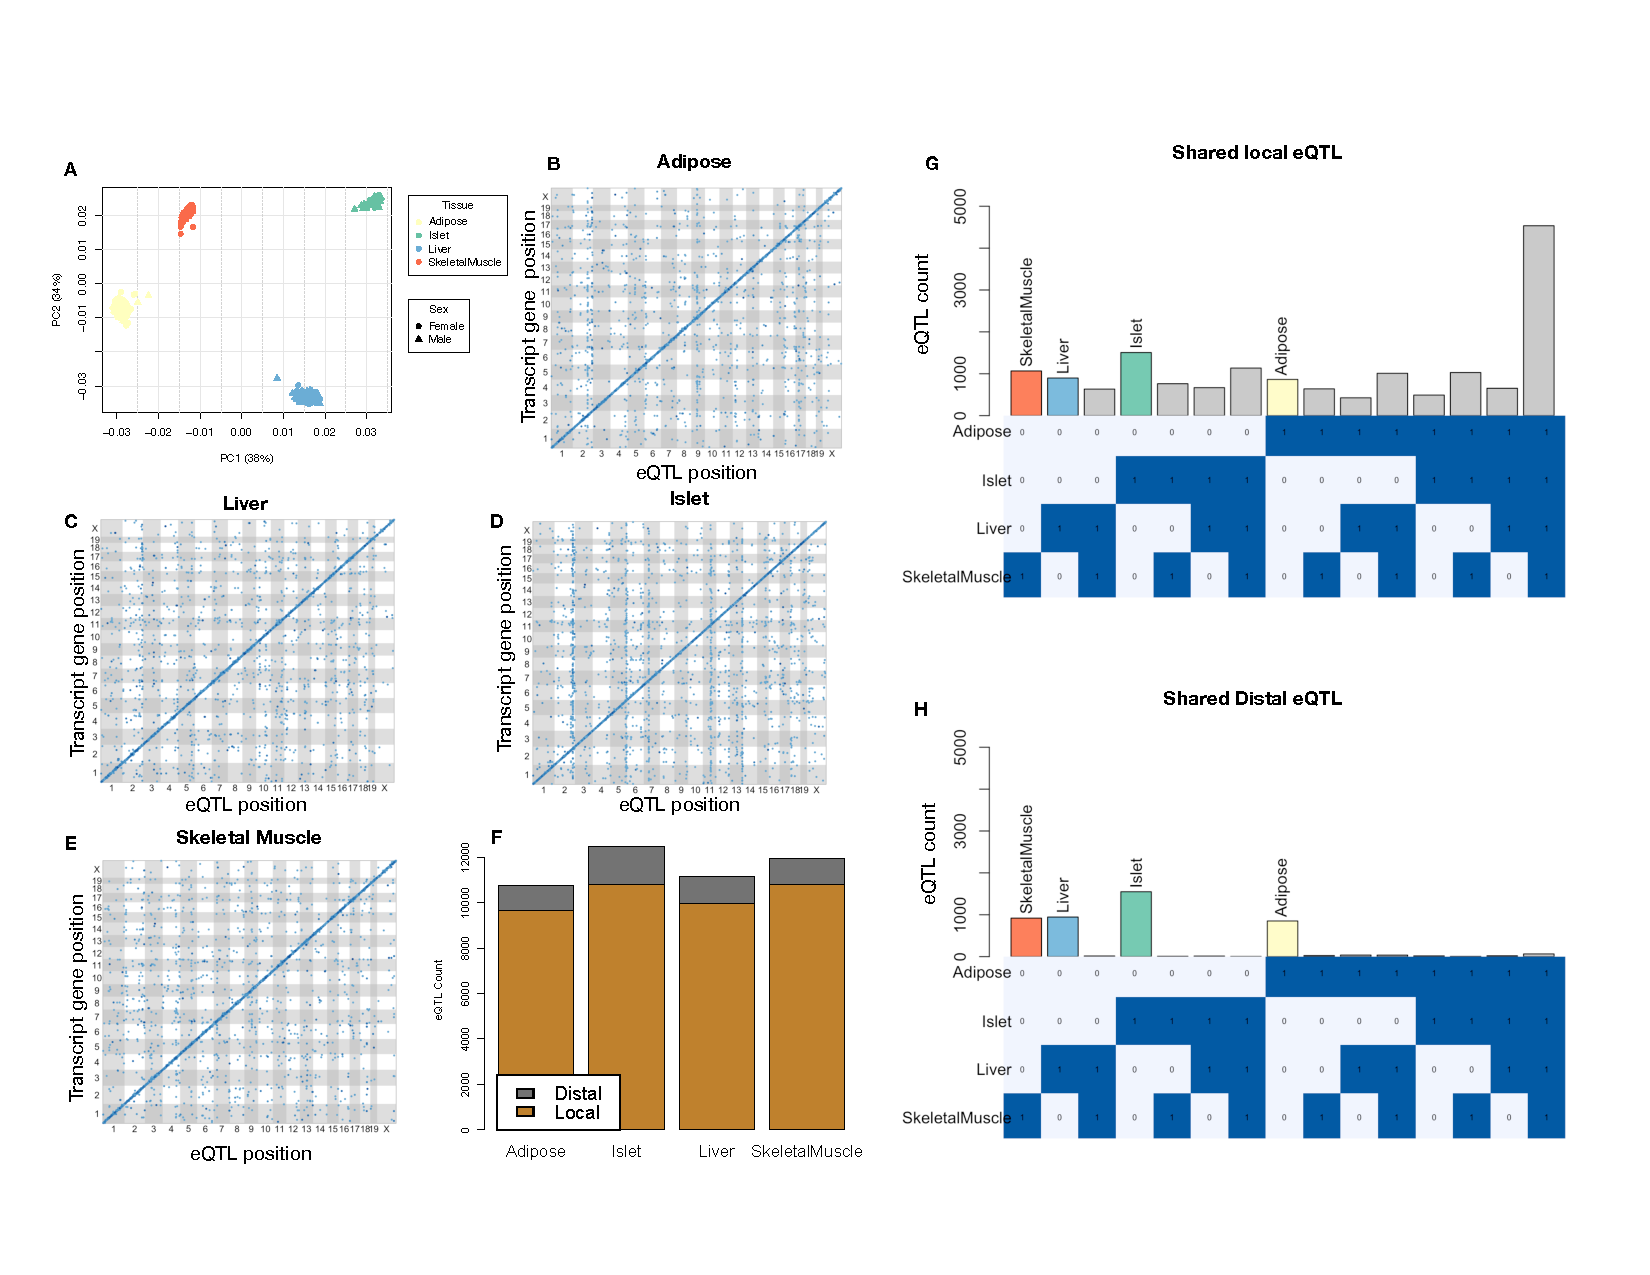
\includegraphics[width=\textwidth]{Figures/Supp_Fig1_eQTL.pdf} 
\caption{Overview of eQTL analysis in DO mice. \textbf{A.} RNA seq 
samples from the four different tissues clustered by tissue. 
\textbf{B.-E.} eQTL maps are shown for each tissue. The $x$-axis 
shows the position of the mapped eQTL, and the $y$-axis shows the 
physical position of the gene encoding each mapped transcript. 
Each dot represents an eQTL with a minimum LOD score of 8. The dots 
on the diagonal are locally regulated eQTL for which the mapped eQTL 
is at the within 4Mb of the encoding gene. Dots off the diagonal are 
distally regulated eQTL for which the mapped eQTL is distant from the 
gene encoding the transcript. \textbf{F.} Comparison of the total number 
of local and distal eQTL with a minimum LOD score of 8 in each tissue. 
All tissues have comparable numbers of eQTL. Local eQTL are much more 
numerous than distal eQTL. \textbf{G.} Counts of transcripts with local 
eQTL shared across multiple tissues. The majority of local eQTL were 
shared across all four tissues. \textbf{H.} Counts of transcripts with 
distal eQTL shared across multiple tissues. The majority of distal eQTL 
were tissue-specific and not shared across multiple tissues. For both G 
and H, eQTL for a given transcript were considered shared in two tissues 
if they were within 4Mb of each other. Colored bars indicate the counts 
for individual tissues for easy of visualization.
}
\label{fig:eQTL}
\end{figure}

\begin{figure}[ht!]
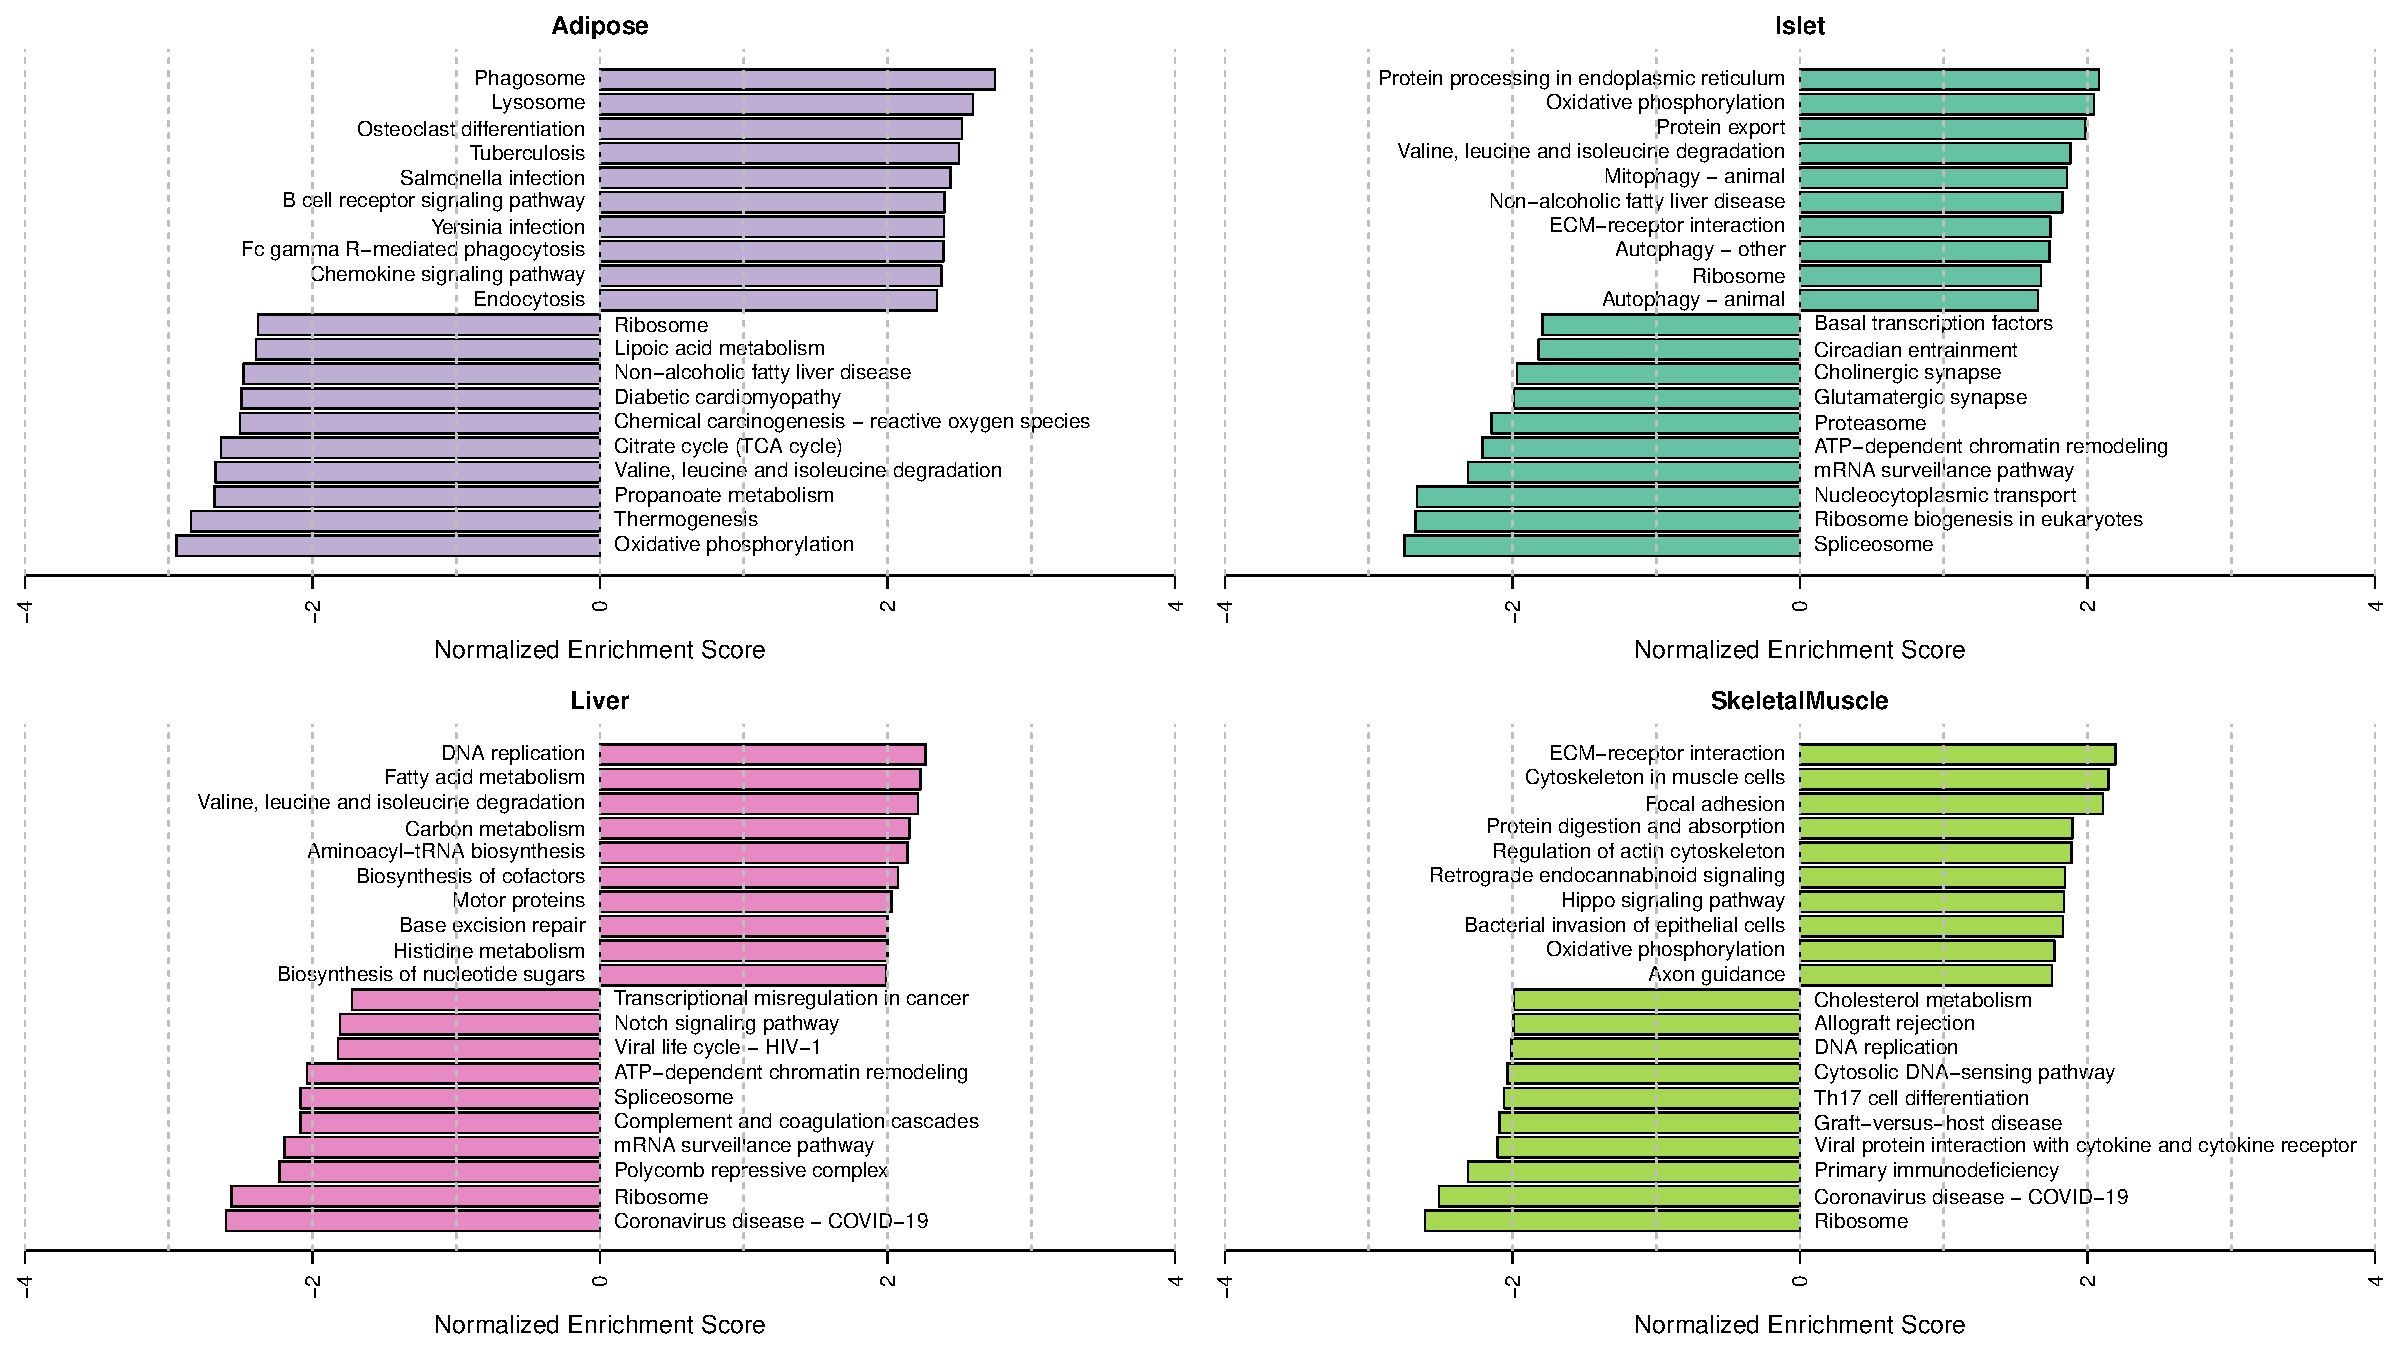
\includegraphics[width=\textwidth]{Figures/Supp_Fig_enrichments_KEGG.pdf} 
\caption{Bar plots showing normalized enrichment scores (NES) for KEGG 
pathways as determined by fast gene score enrichment analysis (fgsea). 
Only the top 10 positive and top 10 negative scores are shown. Colors 
indicate tissue. The name beside each bar shows the name of each enriched 
KEGG pathway.
}
\label{fig:top_enrich_kegg}
\end{figure}

\begin{figure}[ht!]
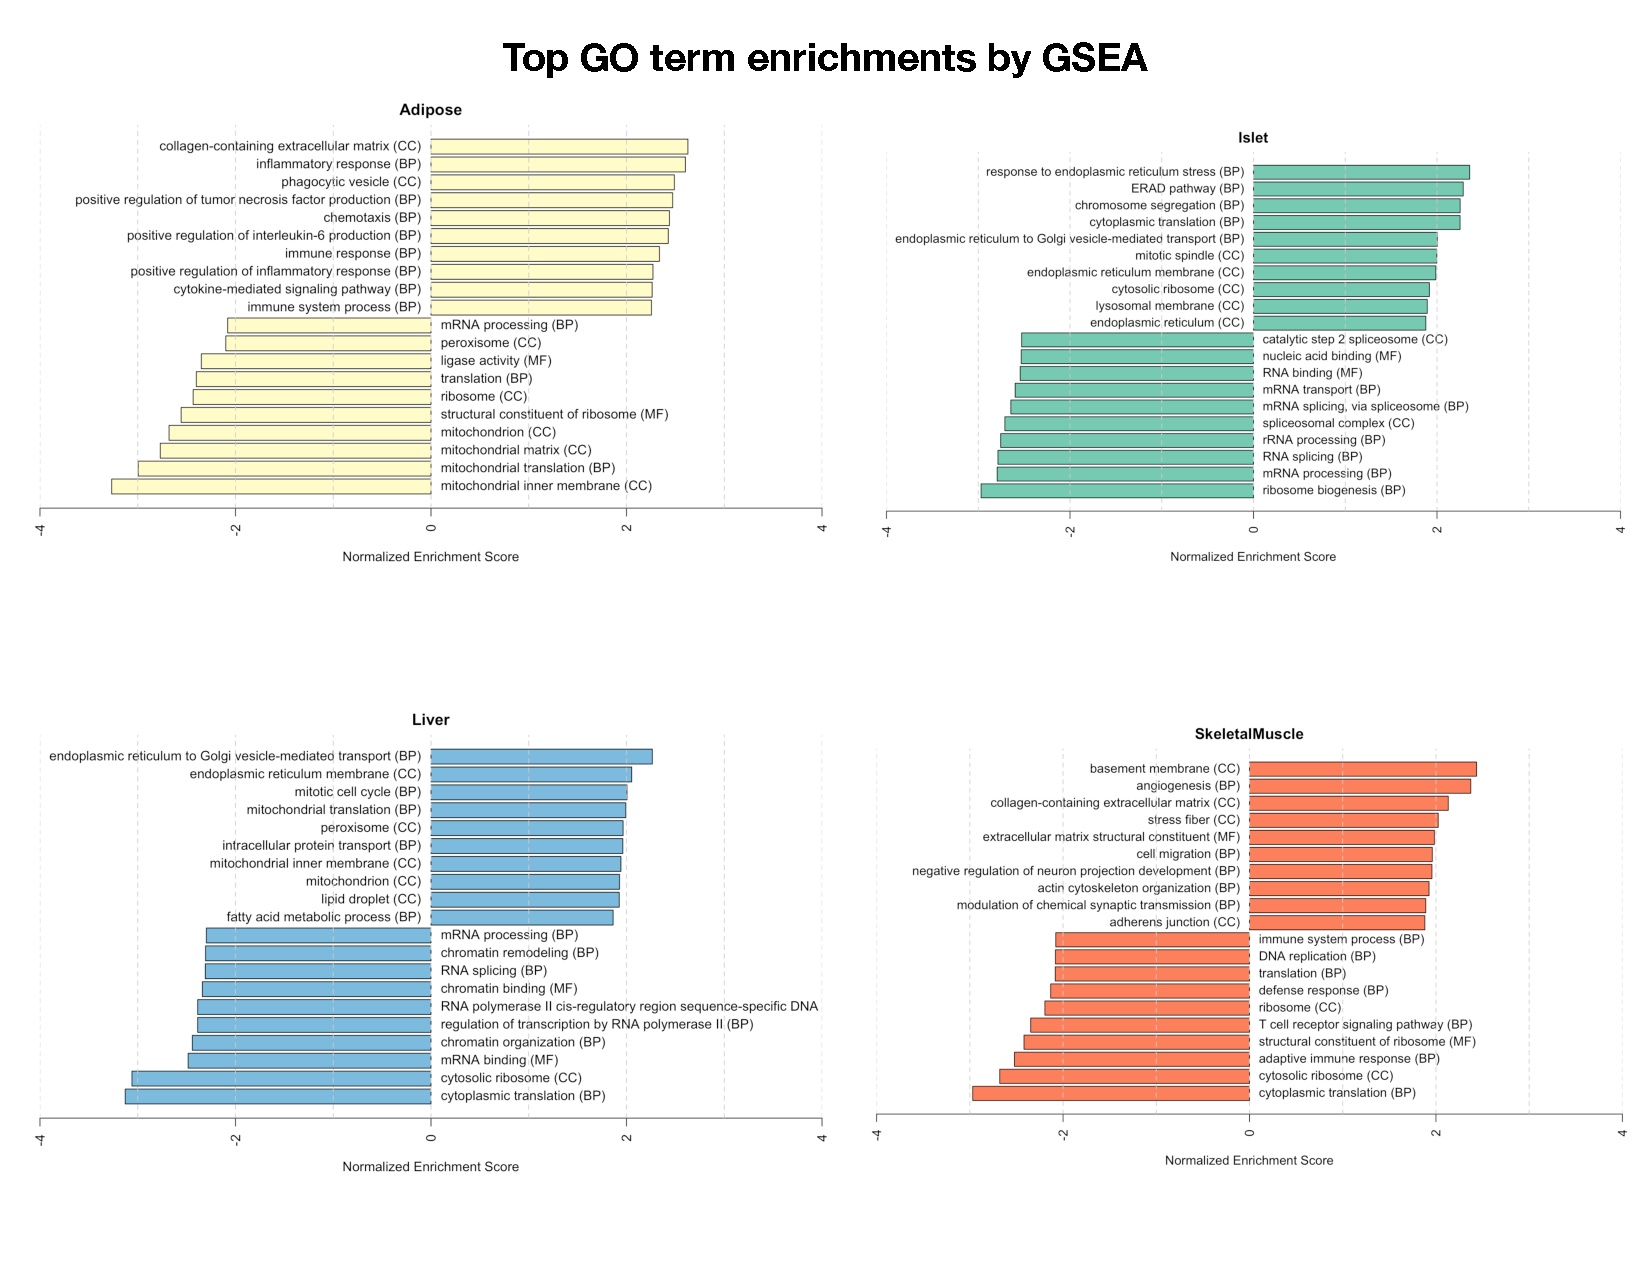
\includegraphics[width=\textwidth]{Figures/Supp_Fig_enrichments_GO.pdf} 
\caption{Bar plots showing normalized enrichment scores (NES) for GO 
terms as determined by fast gene score enrichment analysis (fgsea). 
Only the top 10 positive and top 10 negative scores are shown. Colors 
indicate tissue. The name beside each bar shows the name of each enriched 
GO term. The letters in parentheses indicate whether the term is from the 
biological process ontology (BP), the molecular function ontology (MF), 
or the cellular compartment ontology (CC).
}
\label{fig:top_enrich_go}
\end{figure}

\begin{figure}[ht!]
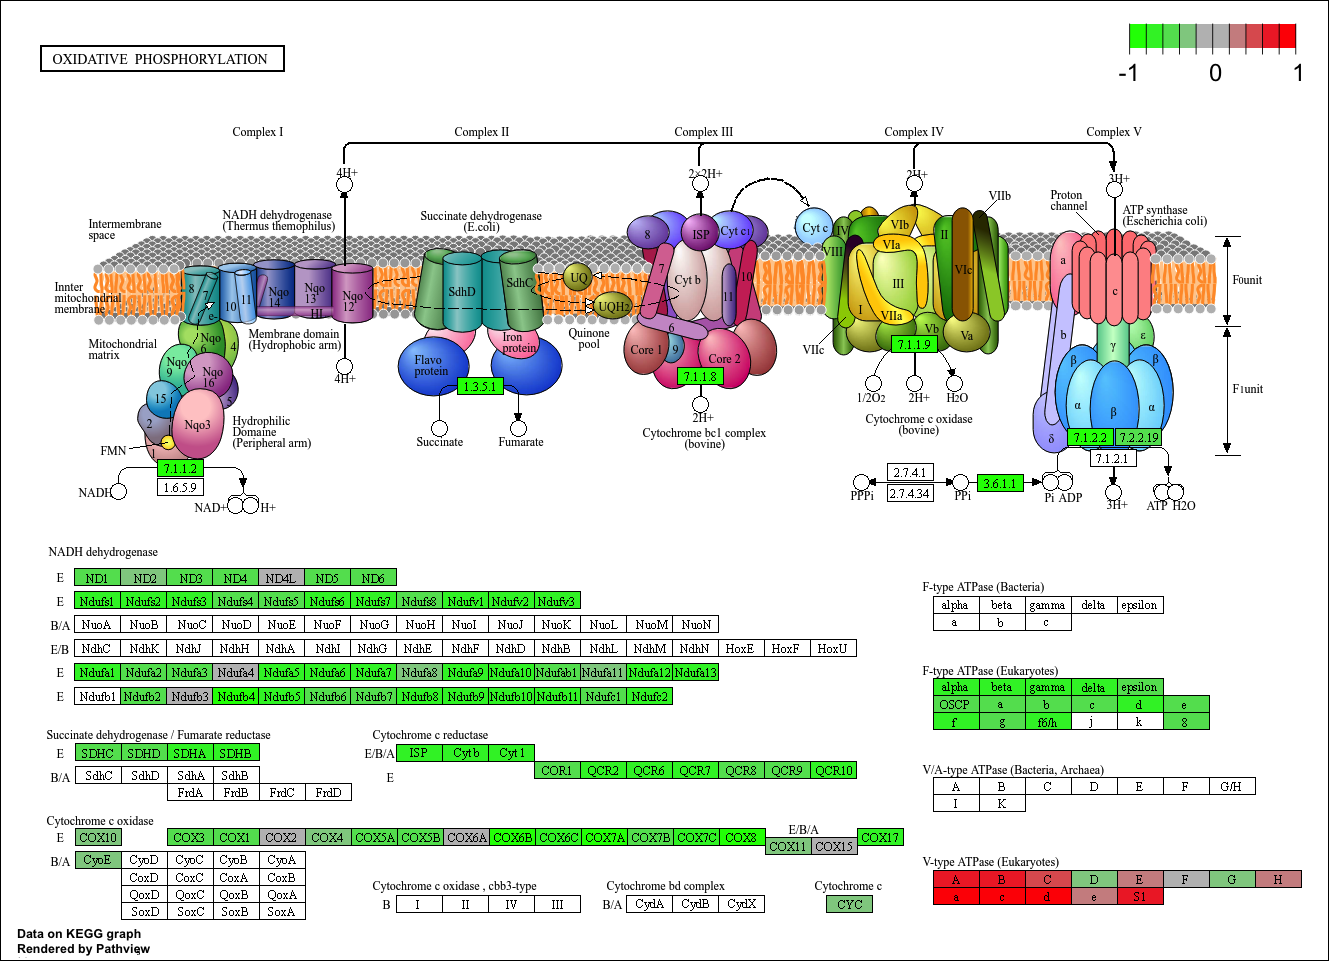
\includegraphics[width=\textwidth]{Figures/Supp_Fig_OxPhos.png} 
\caption{The KEGG pathway for oxidative phosphorylation in 
mice. Each element is colored based on its HDMA loading from adipose
tissue normalized to run from -1 to 1. Genes highlighted in green had 
negative loadings, and those highlighted in red had positive loadings. 
Almost the entire pathway was strongly negatively loaded indicating 
that increased expression of genes involved in oxidative phosphorylation
was associated with reduced MDI.
}
\label{fig:oxPhos}
\end{figure}

\begin{figure}[ht!]
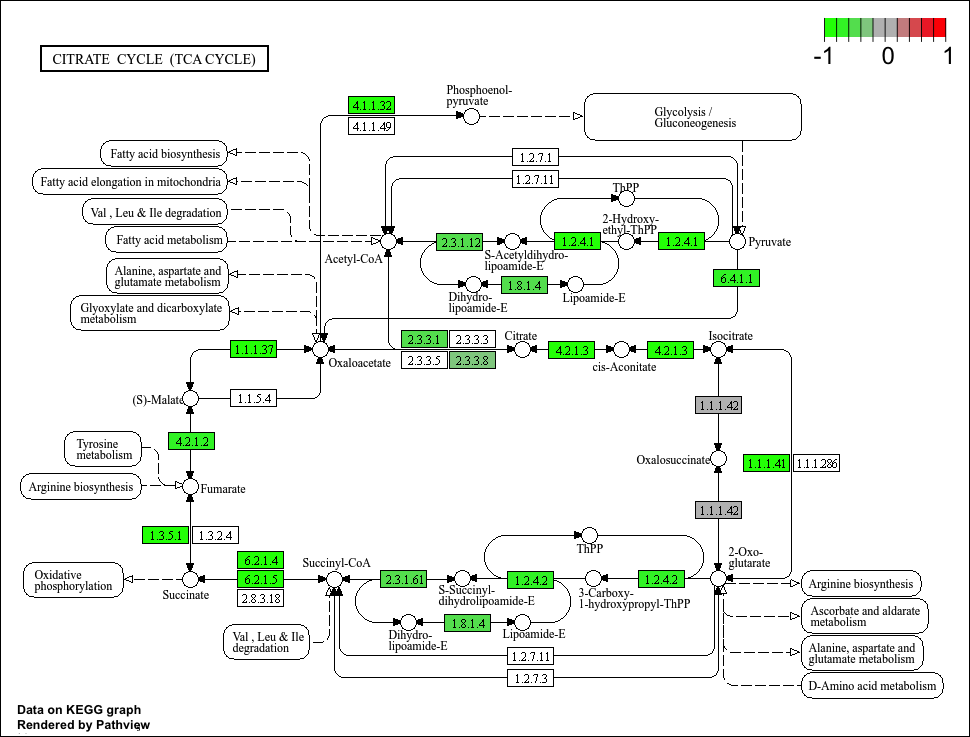
\includegraphics[width=\textwidth]{Figures/Supp_Fig_TCA.png} 
\caption{The KEGG pathway for the TCA (citric acid) cycle in 
mice. Each element is colored based on its HDMA loading from adipose
tissue normalized to run from -1 to 1. Genes highlighted in green had 
negative loadings, and those highlighted in red had positive loadings. 
Many genes in the cycle were strongly negatively loaded indicating 
that increased expression of genes involved in branched-chain amino acid 
degradation was associated with reduced MDI.
}
\label{fig:TCA_cycle}
\end{figure}

\begin{figure}[ht!]
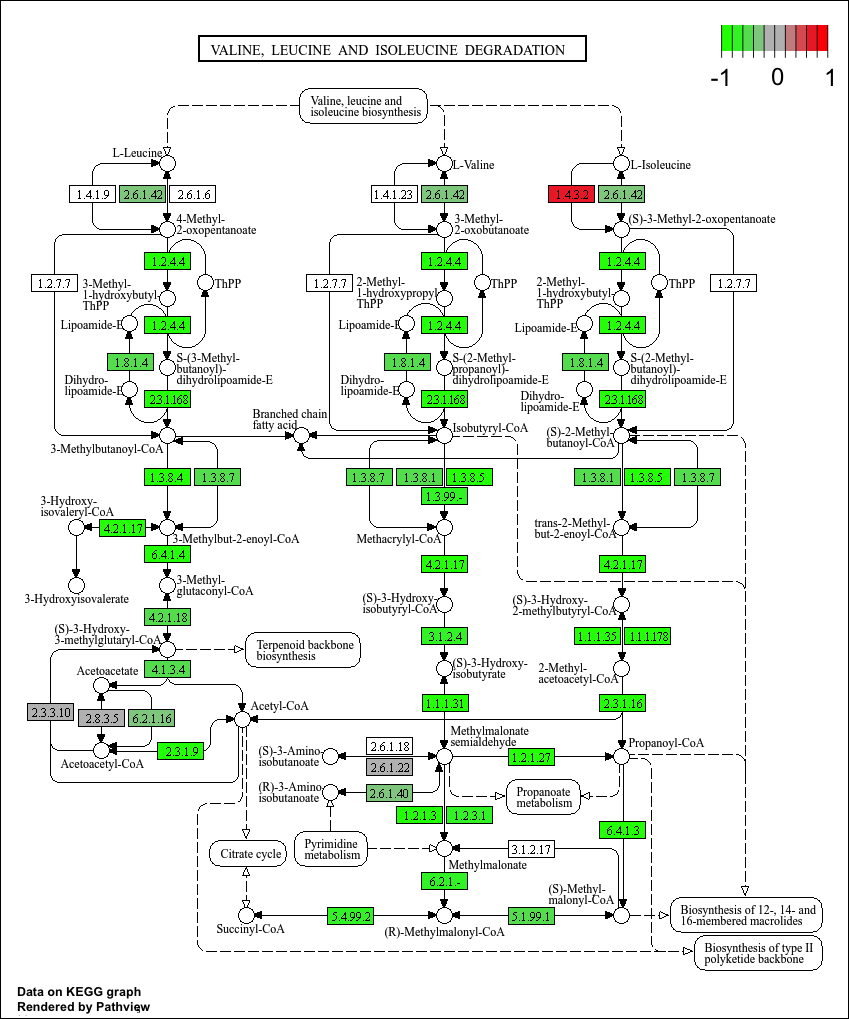
\includegraphics[width=\textwidth]{Figures/Supp_Fig_Branched_Chain.png} 
\caption{The KEGG pathway for branched-chain amino acid degradation in 
mice. Each element is colored based on its HDMA loading from adipose
tissue normalized to run from -1 to 1. Genes highlighted in green had 
negative loadings, and those highlighted in red had positive loadings. 
Almost the entire pathway was strongly negatively loaded indicating 
that increased expression of genes involved in branched-chain amino acid 
degradation was associated with reduced MDI.
}
\label{fig:bcaa_degrataion}
\end{figure}

\begin{figure}[ht!]
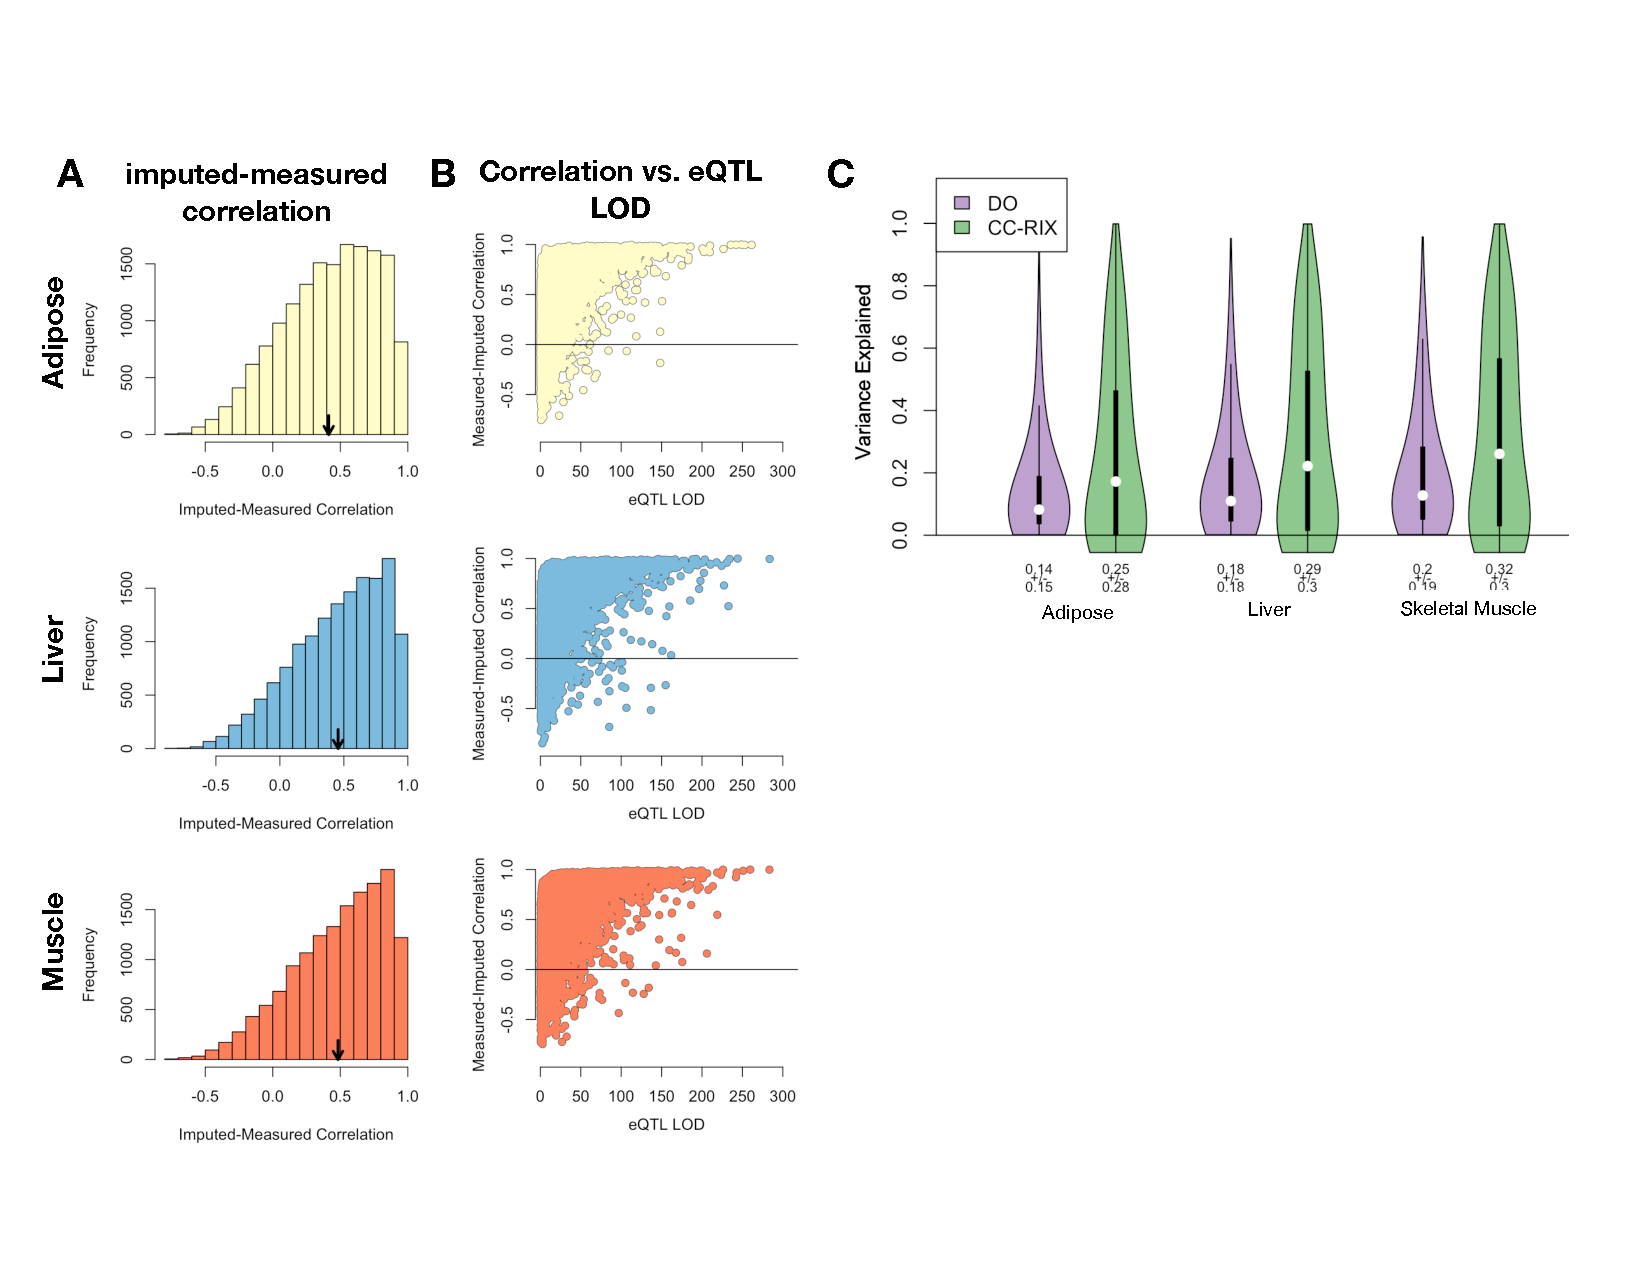
\includegraphics[width=\textwidth]{Figures/Supp_Fig_CC-RIX_Imputation.pdf} 
\caption{Validation of transcript imputation in the CC-RIX. \textbf{A.} 
Distributions of correlations between imputed and measured transcripts 
in the CC-RIX. The mean of each distribution is shown by the red line. 
All distributions were skewed toward positive correlations and had
 positive means near a Pearson correlation (r) of 0.5. \textbf{B.} 
 The relationship between the correlation between measured and 
 imputed expression in the CC-RIX (x-axis) and eQTL LOD score. As 
 expected, imputations are more accurate for transcripts with strong 
 local eQTL. \textbf{C.} Variance explained by local genotype in the 
 DO and CC-RIX. 
}
\label{fig:cc_imputation}
\end{figure}

\begin{figure}[ht!]
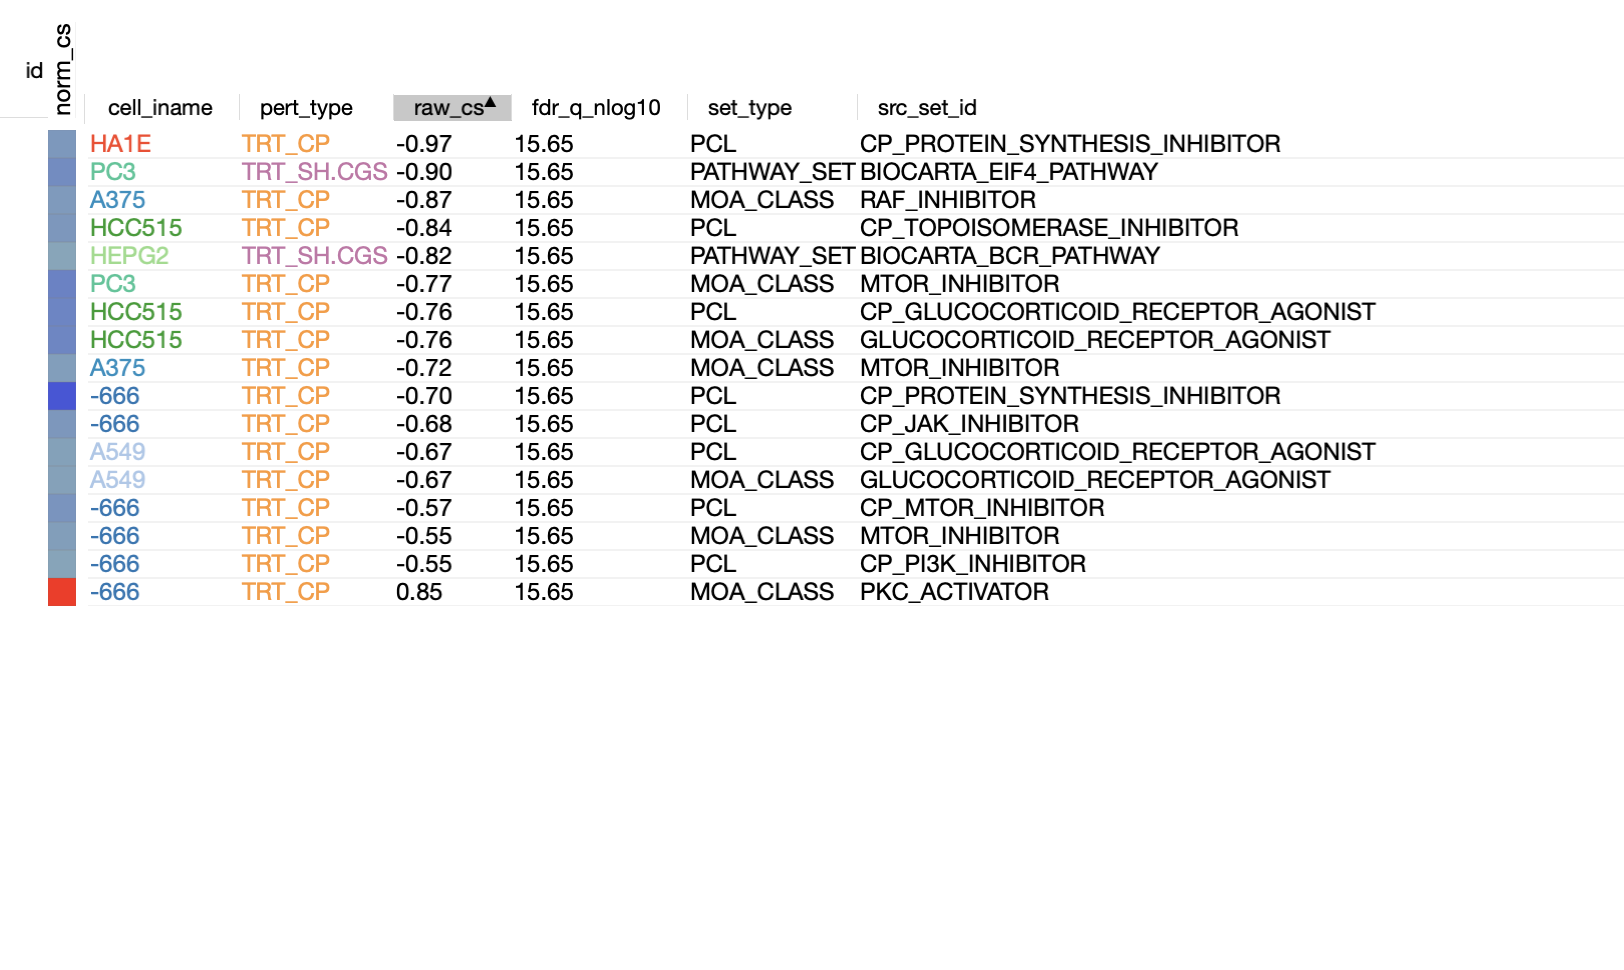
\includegraphics[width=\textwidth]{Figures/Supp_Fig_Adipose_all_cell_types.png} 
\caption{CMAP results using the adipose tissue composite transcript as 
an input. All query results with a $-log_{10}(q) > 15$ across all cell types are 
shown.
}
\label{fig:clue_adipose_all}
\end{figure}

\begin{figure}[ht!]
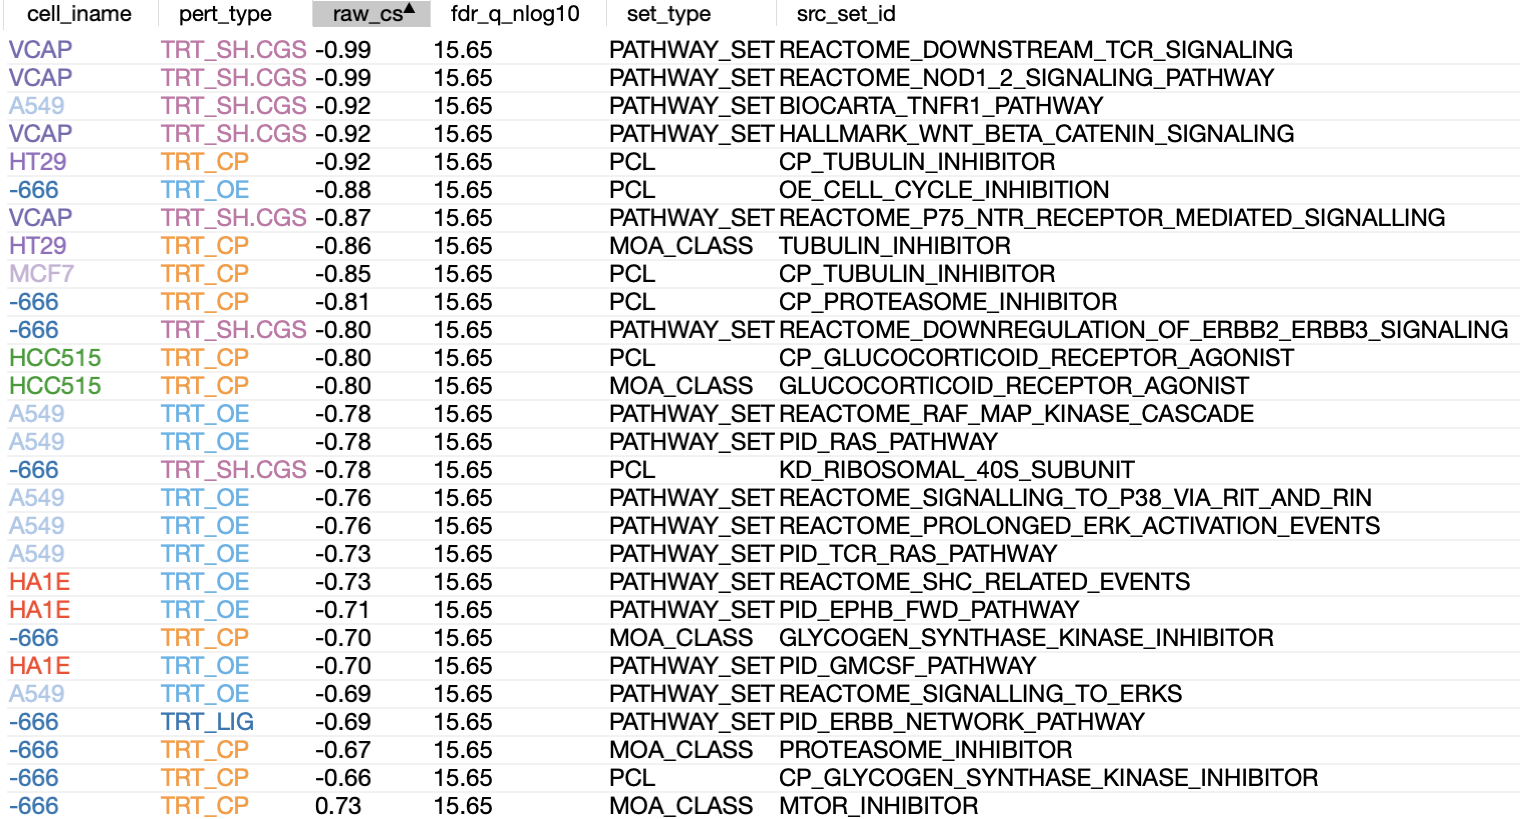
\includegraphics[width=\textwidth]{Figures/Supp_Fig_Islet_all_cell_types.png} 
\caption{CMAP results using the pancreatic islet composite transcript as 
an input. All query results with a $-log_{10}(q) > 15$ across all cell types 
are shown.
}
\label{fig:clue_islet_all}
\end{figure}

\begin{figure}[ht!]
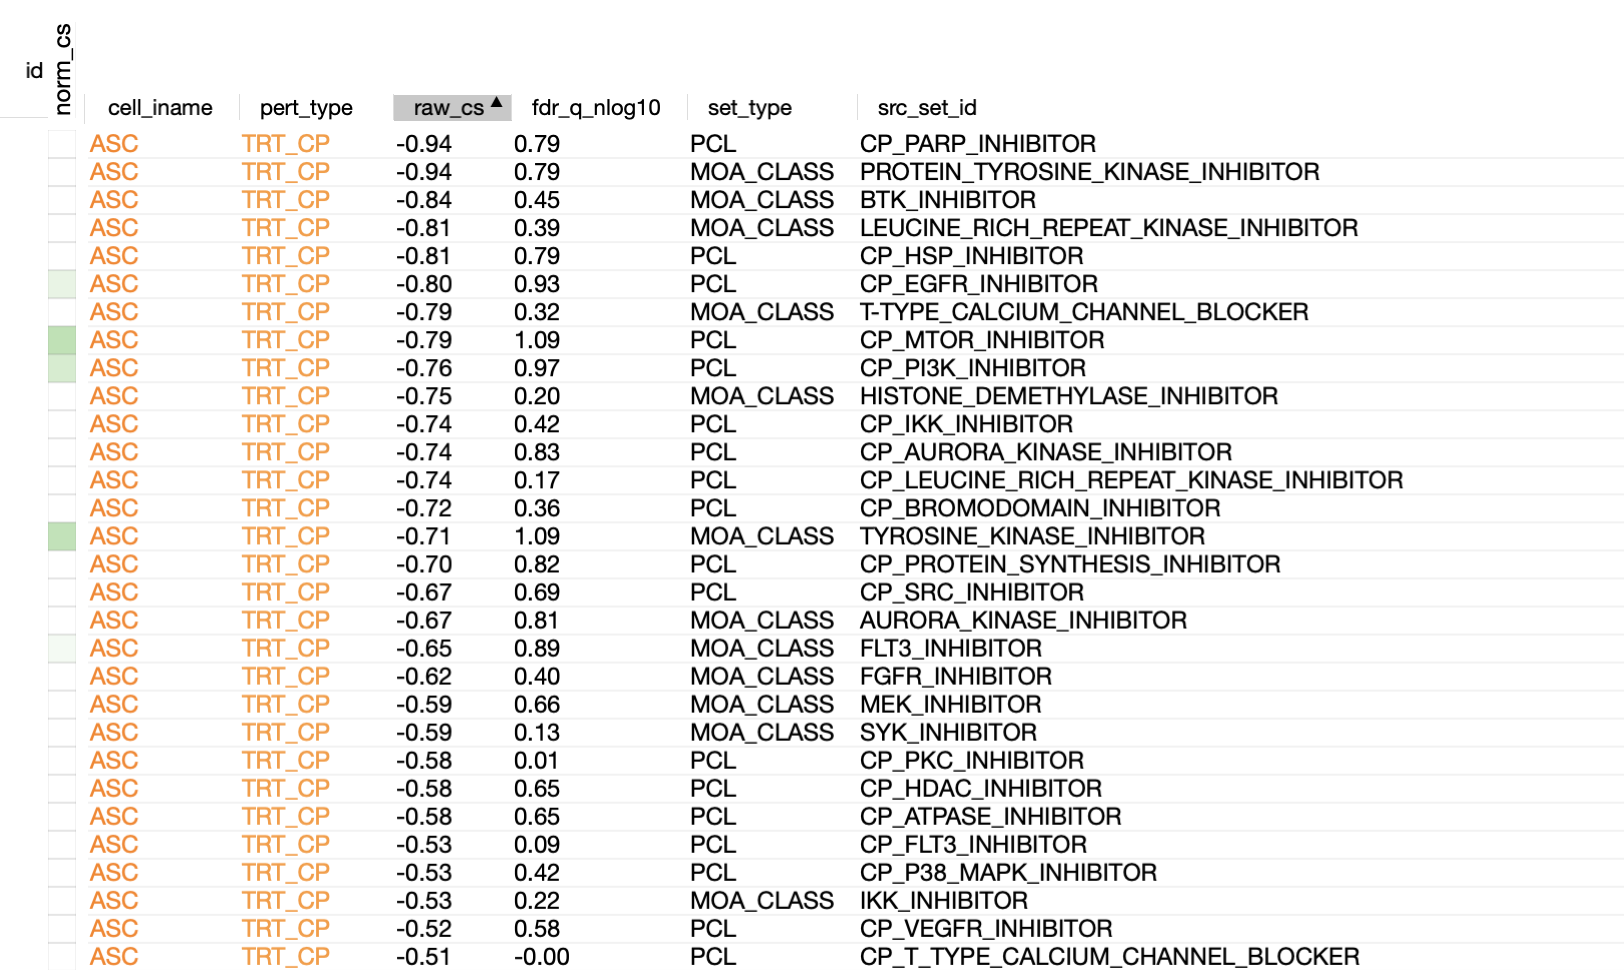
\includegraphics[width=\textwidth]{Figures/Supp_Fig_Adipose_ASC.png} 
\caption{CMAP results using the adipose tissue composite transcript as 
an input. Query results are limited to the 30 most negatively correlated 
signals from normal adipocytes.
}
\label{fig:clue_adipose_asc}
\end{figure}

\begin{figure}[ht!]
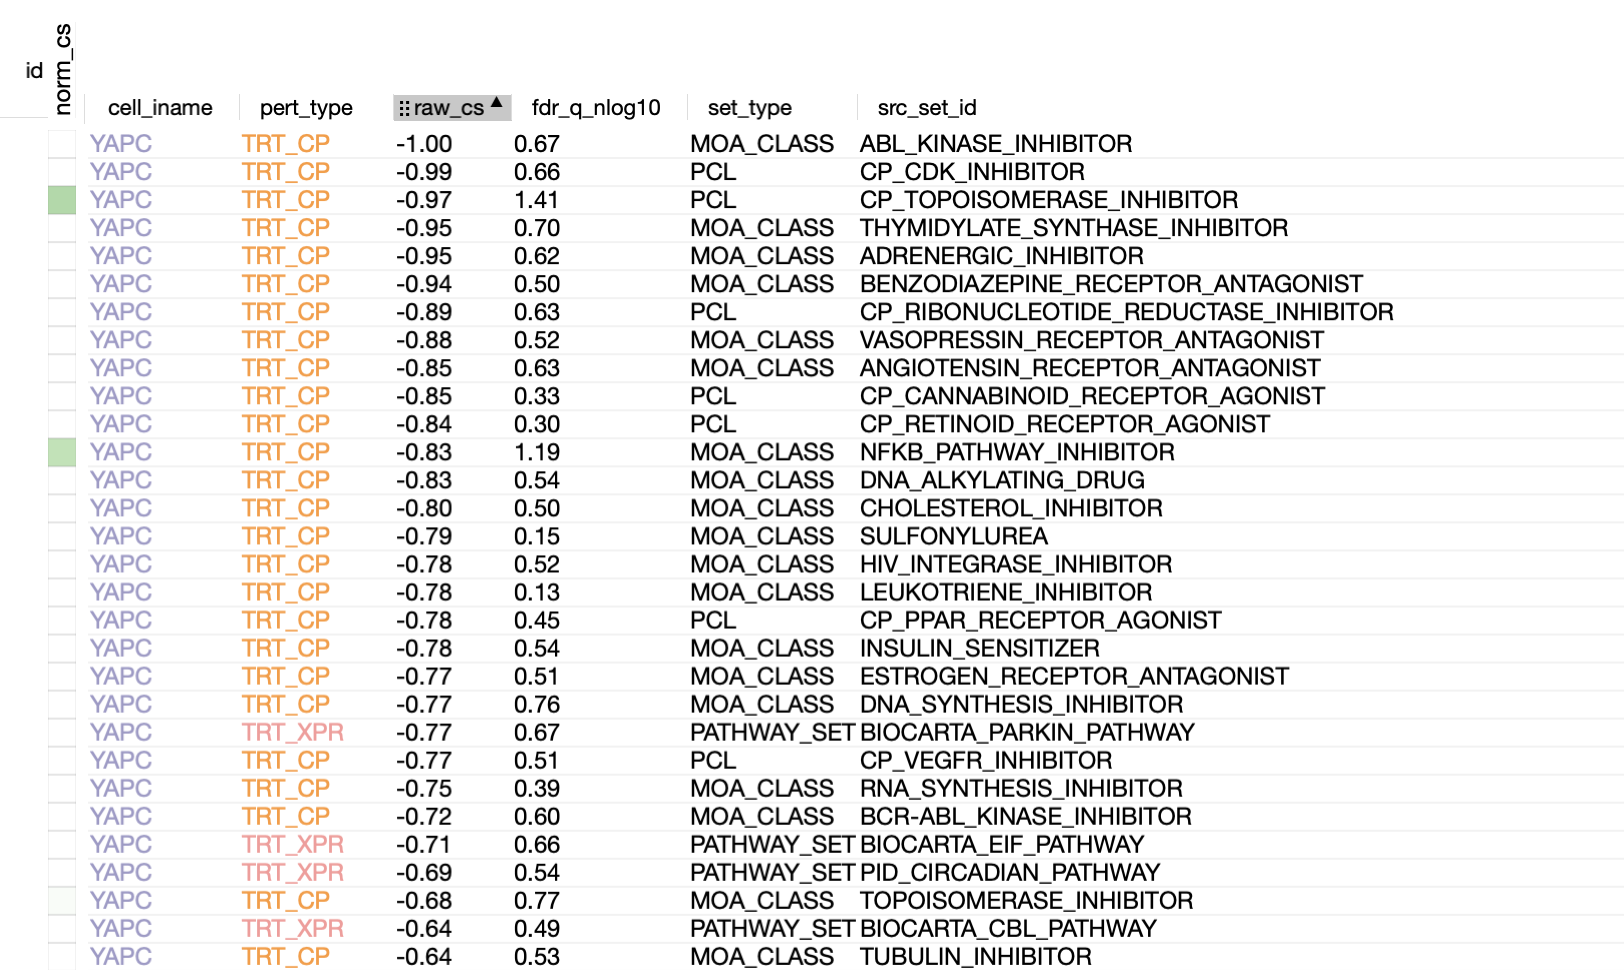
\includegraphics[width=\textwidth]{Figures/Supp_Fig_Islet_YAPC.png} 
\caption{CMAP results using the pancreatic islet composite transcript as 
an input. Query results are limited to the 30 most negatively correlated 
signals from YAPC cells, which were derived from a pancreatic carcinoma cells.
}
\label{fig:clue_islet_yapc}
\end{figure}

\begin{figure}[ht!]
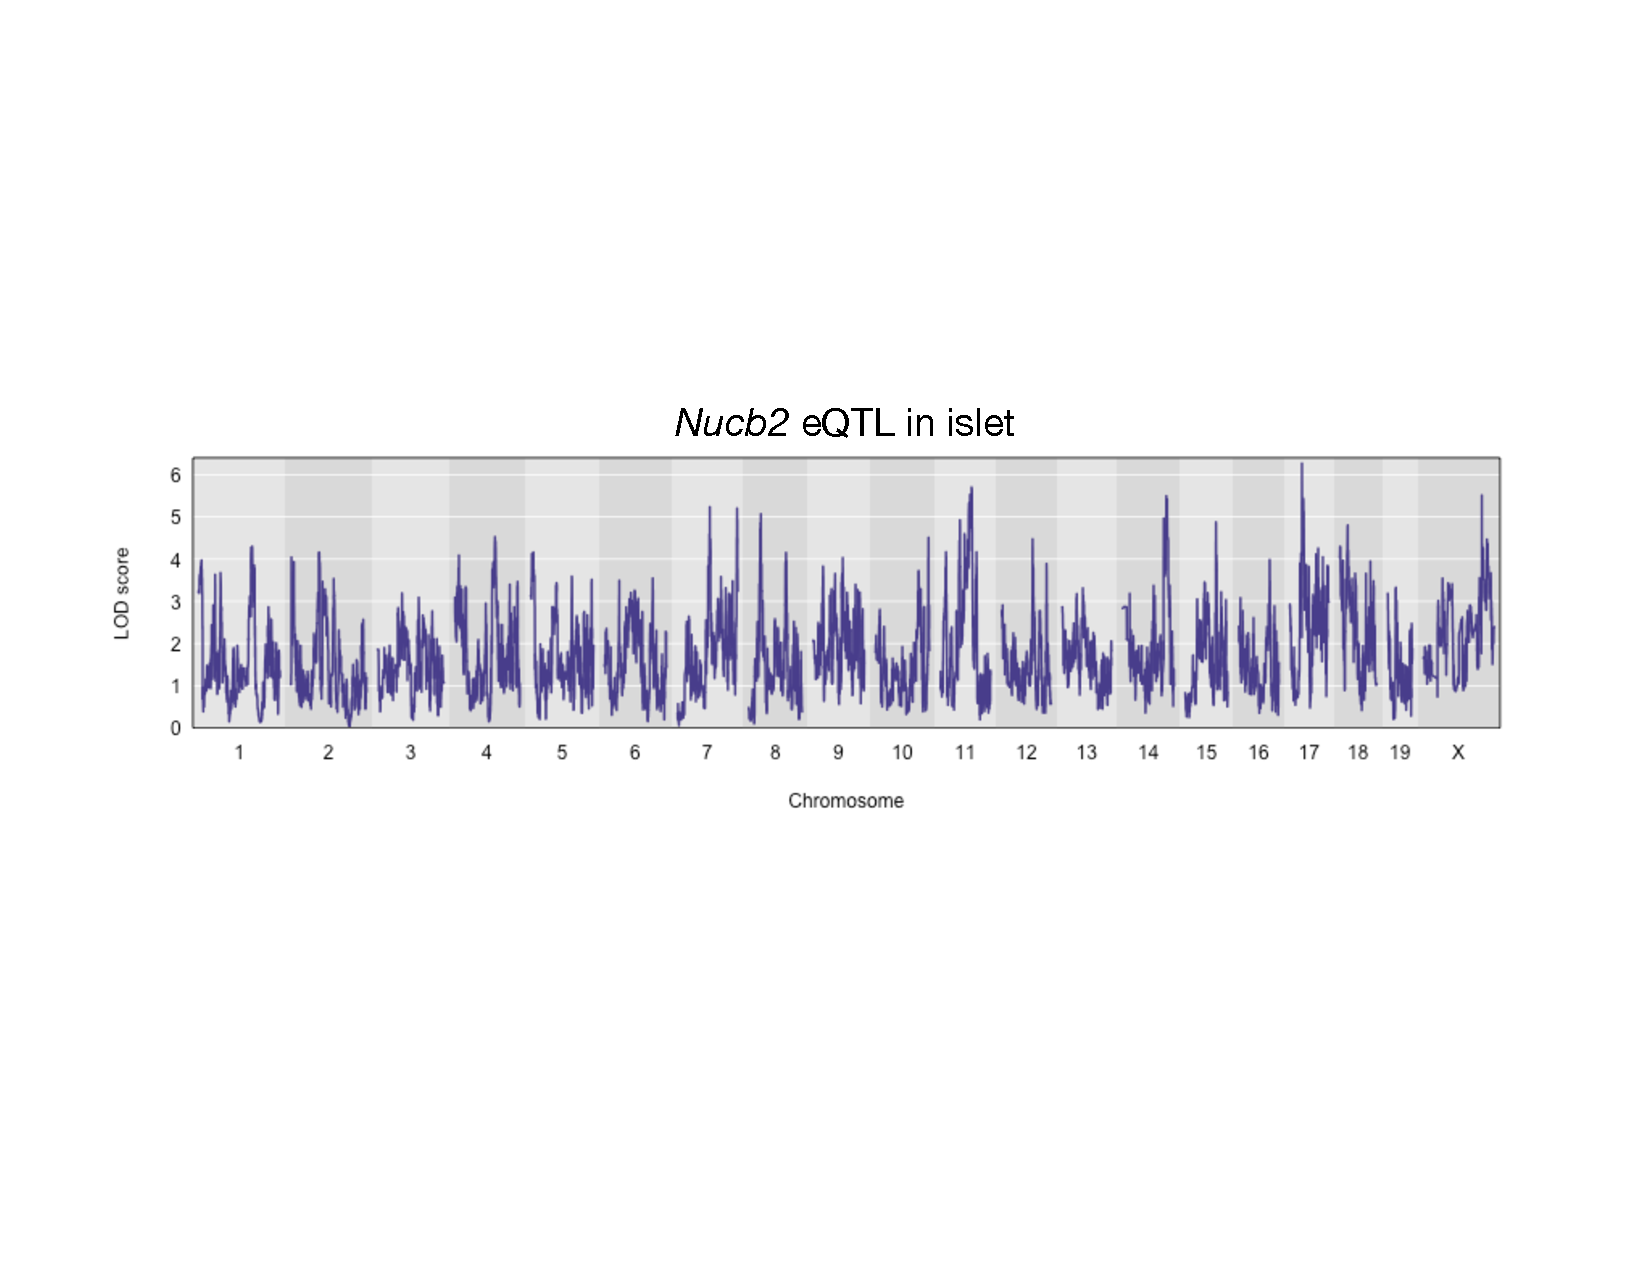
\includegraphics[width=\textwidth]{Figures/Supplemental_FigX_Nucb2_eQTL.pdf} 
\caption{Regulation of \textit{Nucb2} expression in islet. \textit{Nucb2} 
is encoded on mouse chromosome 7 at 116.5 Mb (red line). In islets the 
heritability of \textit{Nucb2} expression levels is 69\% heritable. This 
LOD score trace shows that there is no local eQTL at that position, nor 
any strong distal eQTL anywhere else in the genome. 
}
\label{fig:Nucb2_eqtl}
\end{figure}

\clearpage

\bibliographystyle{unsrt}
\bibliography{islet.bib}

\end{document}
